%----------------------------------------------------------------------------------------
%	PROBLEM 1
%----------------------------------------------------------------------------------------

% To have just one problem per page, simply put a \clearpage after each problem
\newpage
\begin{homeworkProblem}
\section{Ant Colony Optimization}
\subsection{Problem statement}
Implement two stochastic local search (SLS) algorithms for the traveling salesman problem with time windows (TPSTW), building on top of the perturbative local search methods from the first implementation exercise.
\begin{enumerate}
  \item Run each algorithm 25 times with different random seed on each instance. Instances will be available from http://iridia.ulb.ac.be/˜stuetzle/Teaching/HO/. As termination criterion, for each instance, use the maximum computation time it takes to run a full VND (implemented in the previous exercise) on the same instance and then multiply this time by 1000 (to allow for long enough runs of the SLS algorithms).
 \item Compute the following statistics for each of the two SLS algorithms and each instance:
 \begin{itemize}
   \item Percentage of runs with constraint violations
   \item Mean penalised relative percentage deviation
 \end{itemize}

\item Produce boxplots of penalised relative percentage deviation.
\item Determine, using statistical tests (in this case, the Wilcoxon test), whether there is a statistically significant difference between the quality of the solutions generated by the two algorithms.
\item Measure, for each of the implemented algorithms on 5 instances, the run-time distributions to reach sufficiently high quality solutions (e.g. best-known solutions available at http://iridia.ulb.ac.be/˜manuel/tsptw-instances\#instances).
Measure the run-time distributions across 25 repetitions using a cut-off time of 10 times the termination criterion above.
\item Produce a written report on the implementation exercise:
\begin{itemize}
  \item Please make sure that each implemented SLS algorithm is appropriately described and that the computational results are carefully interpreted. Justify also the choice of the parameter settings and the choice
of the iterative improvement algorithm for the hybrid SLS algorithm.
  \item Present the results as in the previous implementation exercise (tables, boxplots, statistical tests).
  \item Present graphically the results of the analysis of the run-time distributions.
  \item Interpret appropriately the results and make conclusions on the relative performance of the algorithms across all the benchmark instances studied.
\end{itemize}
\end{enumerate}

\subsection{Introduction} \label{sec:intro}
Ant Colony Optimization is an example of population-based metaheuristic (i.e a set of algorithmic concepts that can be used to define heuristic methods) inspired by the behavior of the ant species \emph{Iridomyrmex humilis}.

To be more precise, these insects are able, by means of stigmergic communication, to choose the shortest path between their nest and a food source, when given the choice (\cite{deneubourg1990self}).

The communication process occurs by deposing a certain quantity of pheromone in the environment that can be sensed by the other ants and that will be used by them as an heuristic (i.e an information to guide their choice) for selecting the shortest path.

Furthermore, the pheromone quantity on a certain location decreases over time because of evaporation, thus requiring a continuous deposit process to be effective.

The convergence to one of the paths will occur as a consequence of the self-reinforcing pheromone deposit mechanism.
In fact the more pheromone is deposited on a path, the more ants will follow the pheromone trail on that path deposing even more pheromone.

The first application of Ant Colony Optimization method, the Ant System, has been made on the optimization version of the Travelling Salesman Problem (TSP) (\cite{dorigo1996ant}).

In this implemetation a population of virtual agents (an ant colony) is used to explore the search space (the virtual environment).

In the same fashion as the real insects, the ants are able to deposit virtual pheromone in the environment, to signal to the other ants the presence of promising solutions.

The general outline of the implemented algorithm is the following (as in \cite{dorigo2006artificial}):

\begin{algorithm}[!h]
  \caption{Ant Colony Optimization - Outline}\label{aco}
  \begin{algorithmic}[1]
    \State \emph{InitalizePheromoneTrail} 
    \While{!(TerminationCondition)}
        \State \emph{ConstructAntsSolutions}
        \State \emph{LocalSearch} (Optional)
        \State \emph{UpdatePheromoneTrails}
    \EndWhile
\end{algorithmic}
\end{algorithm}



\subsection{Problem formulation}
An instance of the Travelling Salesman Problem with Time Windows (TSPTW) can be expressed as a tuple $<N,E,c,t>$ where:
\begin{itemize}
  \item $N:\{0,\cdots,n\}$ - Node set 
  \item $E:N\times N$ - Edge set
  \item $c:E\mapsto \mathbb{R}$ - Edge cost function mapping a cost $c$ to every edge $e \in E$. 
  \item $t:N\mapsto \mathbb{R}^2$ - Time window function mapping a couple of values $a_i,b_i$ representing respectively, the opening and closing time of the time window, such that $a_i<b_i$, to every node $i \in N$.
  \item A candidate solution for the problem, in this case, is represented as a permutation $p$ of the nodes in $N$, where $p_i$ represents the $i^{th}$ solution component (node) in the sequence, such that $p_0 = 0 \forall p$.
\end{itemize}

As in \cite{lopez2010beam} the formal definition of the problem is:
\begin{equation} \label{eq:probform}
 \begin{array}{rl}
  \textbf{min} & f(p)= \sum\limits_{i=0}^{n} c(e_{p_{i}p_{k+i}}) \\
  \textbf{subject to} & \Omega(p)= \sum\limits_{i=0}^{n+1} \omega(p_{i}) = 0
 \end{array}
\end{equation}

where

\begin{equation} \label{eq:cv}
\begin{array}{c}
 \omega(p_{i}) \begin{cases}
                1 & A_{p_i} < b_{p_i}  \\
                0 & \text{otherwise} \\   
               \end{cases} \\
 A_{p_{i+1}} = \max(A_{p_i},a_i) + c(e_{p_{i}p_{k+i}}) 
\end{array}
\end{equation}

As one may notice in \ref{eq:probform} and \ref{eq:cv}, a feasible solution $p$ for the problem is a permutation where the constraints related to the time windows are met for every node $i$ in the permutation.

\subsection{Algorithm structure}
The proposed algorithm is an implementation of one of the extensions to the Ant Colony Optimization metaheuristic framework, the \maxmin Ant System (cf. \cite{stutzle2000max}).
The main features of the algorithm are the following:
\begin{itemize}
  \item Only iteration best or best-so-far ants update pheromone
  \item $\forall t \text{ } \tau_{\min} < \tau_{i,j}(t) < \tau_{\max}  $ - Pheromone trails have explicit upper and lower limits
  \item $\tau_{i,j}(0) = \tau_0 = \tau_{\max}$ - Pheromone trails initialized to upper limit
  \item Pheromone trails are re-initialized when stagnated
\end{itemize}

\begin{algorithm}[!h]
  \caption{\maxmin Ant System for TSPTW - Outline}\label{maxmintsptw}
  \begin{algorithmic}[1]
    \Procedure{ACO}{$\alpha,\beta,\rho,\tau_0,q_0,n_{ants},n_{cities},t_{max}$}\Comment{The main procedure}
    \Require $N$ - Node set
    \Require $E$ - Edge set 
    \Require $c$ - Edge cost function
    \Require $t$ - Time window function
    \State {\emph{InitalizePheromoneTrail}($\tau_0,n_{cities}$)}
    \While{\emph{!TerminationCondition}($t_{max}$)}
      \ForAll {Ants}
        \State \emph{ConstructSolution}($\alpha,\beta$)
        \State \emph{IterativeImprovement}(INSERT,BEST-IMPROVEMENT)
        \State \emph{UpdatePheromoneTrails}($\rho,q_0$)
      \EndFor
    \EndWhile
    \State \textbf{return} solution
    \State
  \EndProcedure
\end{algorithmic}
\end{algorithm}

\begin{minipage}{.45\textwidth}
\centering
\begin{tikzpicture}[->,>=stealth',shorten >=1pt,auto,node distance=3cm,
                    semithick]
  \tikzstyle{every state}=[fill=blue!20,draw=none,thick]

  \node[initial,state] (Init)                    {};
  \node[state]         (CI) [right of=Init]     {\emph{CI}};
  \node[state]         (CS) [above right of=CI] {\emph{CS}};
  \node[state]         (LS) [below right of=CI] {\emph{LS}};

  \path (Init) edge              node {DET:\emph{IPT}()} (CI)
        (CI) edge              node {DET} (CS)
        (CS) edge [loop above] node {CDET(not \emph{SC})} (CS)
            edge              node {CDET(\emph{SC})} (LS)
        (LS) edge [loop below] node {CDET(not \emph{LO})} (LS)
            edge               node {CDET(\emph{LO})} (CI);
\end{tikzpicture}
\captionof{figure}{\maxmin Ant System GLSM}
\end{minipage}%
\hspace{1.5cm}
\begin{minipage}{.45\textwidth}
\centering
\begin{itemize}
  \item \emph{IPT}() $\equiv$ \emph{InitializePheromoneTrail}()
  \item \emph{SC} $\equiv$ \emph{SolutionComplete}()
  \item \emph{LO} $\equiv$ \emph{LocalOptimum}()
\end{itemize}
\end{minipage}

In the implementation, an instance is completely defined by:
\begin{itemize}
\item \textbf{Cost matrix} - Encapsulating information on the node set $N$, edge set $E$, and weighting of each edge $c$.
\item \textbf{Time window vector} - Describing the time window mapping function $t$ for each node.
\end{itemize}

\subsubsection{Pheromone Initialization}
As discussed in \ref{sec:intro}, the ACO methods are based on stigmergic communication among the agents by means of virtual pheromone.

While the real ants can deposit pheromone anywhere in the environment, the virtual ants may only exchange informations concerning solutions components.

For this reason, every admissible edge $e_{ij}$ of $E$ has an associated pheromone value $\tau_{ij}$, that have to be initialized at the beginning of the execution of the algorithm.

The inizialization value $\tau_0$ is a parameter of the algorithm.

\begin{algorithm}[!h]
  \caption{Pheromone Initialization}\label{init}
  \begin{algorithmic}[1]
    \Procedure{InitalizePheromoneTrail}{$\tau_0,n_{cities}$}
      \State $\tau_{\max} \gets $
      \State $\tau_{\min} \gets $
      \State $i \gets 0$
      \State $j \gets 0$
      \For{$i < n_{cities}$} 
        \For{$j < i$} 
          \State $\tau_{ij} \gets \tau_0$
          \State $\tau_{ji} \gets \tau_{ij}$
          \State $ j \gets j + 1$  
        \EndFor
        \State $ i \gets i + 1$ 
      \EndFor
    \EndProcedure
\end{algorithmic}
\end{algorithm}

\subsubsection{Solution construction}
\begin{algorithm}[!h]
  \caption{Solution Construction}\label{sol}
  \begin{algorithmic}[1]
    \Procedure{ConstructSolution}{$\alpha,\beta$}\Comment{The main procedure}
      \State \Comment{$s_i$ reprents the $i^{th}$ component of the solution}
      \State $s_0 \gets 0$ \Comment{Every solution starts at the depot}
      \State $s_1 \gets$ \emph{RandomCitySelection}() \Comment{Random choice of the starting city}
      \State $i \gets 1$
      \While{!\emph{SolutionComplete}()}
        \State $k \gets $ \emph{RouletteWheelSelection}() \Comment{ $k$ stochastically chosen according to the probability distribution defined by $p_k$}
        \State $s_i \gets k$ 
        \State $i \gets i+1$
      \EndWhile
    \EndProcedure
\end{algorithmic}
\end{algorithm}

\begin{equation}
p_k = \begin{cases}
  \frac{[\tau_{i-1,k}]^\alpha \cdot [\eta_{i-1,k}]^\beta}{\sum_{j \in N(s_{i-1})} [\tau_{i-1,j}]^\alpha \cdot [\eta_{i-1,j}]^\beta} & k \in N(s_{i-1}) \\
 0 & \text{otherwise} \\
\end{cases}
\end{equation}

\subsection{Possible heuristics}
\subsubsection{Cheng and Mao, 2007}
The local heuristics used in the current algorithm are similar to that proposed by Gambardella et al. [24] in their
multiple ant colony system (MACS) designed to solve the vehicle routing problem with time windows (VRPTW).

[24]  L.M. Gambardella, E.D. Taillard, G. Agazzi, MACS-VRPTW: A multiple ant colony system for vehicle routing problems with time windows,
in: D. Corne, M. Dorigo, F. Glover (Eds.), New Ideas in Optimization, McGraw Hill, London, UK, 1999, pp. 63–76.

\begin{equation}
[\eta_{i-1,k}]^\beta = [g_{i-1,k}]^\beta \cdot [h_{i-1,k}]^\gamma
\end{equation}  

\begin{equation}
g_{i-1,k} = \begin{cases}
 \frac{1}{1+e^{\delta \cdot (G_{i-1,k} - \mu)}}  &  G_{i-1,k} = b_k - t_k \geq 0 \\
0 & \text{otherwise} \\
\end{cases}
\end{equation}
where
\begin{itemize}
  \item $G_{i,j} = b_j - t_j$ - Slack corresponding to the time window $j$ while being in node $i$
  \item $t_i$ - Arrival time at node $i$
  \item $b_i$ - Closing time of time window $i$
  \item $G(i) = \{k\text{ } | \text{ }G_{i,k} \geq 0\}$ - Set of feasible neighbors of node $i$ (i.e. such that node $k$ is reached earlier than its closing time)
  \item $\mu = \frac{1}{|G(i)|}\sum_{j \in G(i)}  G_{i,j}$ - Average slack 
  \item $\delta$ - Parameter to control the slope of the sigmoidal function
\end{itemize}

\begin{equation}
h_{i-1,k} = \begin{cases}
 \frac{1}{1+e^{\lambda \cdot (H_{i-1,k} - \upsilon)}}  &  H_{i-1,k} = t_k - a_k \geq 0 \\
0 & \text{otherwise} \\
\end{cases}
\end{equation}
where
\begin{itemize}
  \item $H_{i,j} = t_j - a_j$ - Waiting time corresponding to the time window $j$ while being in node $i$
  \item $t_i$ - Arrival time at node $i$
  \item $a_i$ - Opening time of time window $i$
  \item $H(i) = \{k\text{ } | \text{ }H_{i,k} \geq 0\}$ - Set of non-waiting neighbors of node $i$ (i.e such that node $k$ is reached within the time window)
  \item $\upsilon = \frac{1}{|H(i)|}\sum_{j \in H(i)}  H_{i,j}$ - Average waiting time 
  $\lambda$ - Parameter to control the slope of the sigmoidal function 
\end{itemize}


\subsubsection{Lopez-Ibanez and Blum, 2009}

\begin{equation}
\eta_{i-1,k} = \lambda_{a} \cdot \frac{a_{\max}-a_{k}}{a_{\max}-a_{\min}} + \lambda_{b} \cdot \frac{b_{\max}-b_{k}}{b_{\max}-b_{\min}} + \lambda_{c} \cdot \frac{c_{\max}-c_{i-1,k}}{c_{\max}-c_{\min}}
\end{equation}

where
\begin{itemize}
  \item $a_i$ - Opening time of time window $i$
  \item $a_{\max} = \max_{j \in N(i)} a_{j}$ - Maximum time window opening time in the neighborhood of node $i$
  \item $a_{\min} = \min_{j \in N(i)} a_{j}$ - Minimum time window opening time in the neighborhood of node $i$
  \item $b_i$ - Closing time of time window $i$
  \item $b_{\max} = \max_{j \in N(i)} b_{j}$ - Maximum time window closing time in the neighborhood of node $i$
  \item $b_{\min} = \min_{j \in N(i)} b_{j}$ - Minimum time window closing time in the neighborhood of node $i$
  \item $c_{i,j}$ - Travelling cost from node $i$ - $j$
  \item $c_{\max} = \max_j c_{i,j}$ - Maximum travelling cost from node $i$ 
  \item $c_{\min} = \min_j c_{i,j}$ - Minimum travelling cost from node $i$
  \item $\lambda_{a},\lambda_{b},\lambda_{c}$ such that $\lambda_{a}+\lambda_{b}+\lambda_{c}=1$ - Randomly picked weights
\end{itemize}


\begin{algorithm}[!h]
  \caption{Pheromone Trails Update}\label{update}
  \begin{algorithmic}[1]
    \Procedure{UpdatePheromoneTrails}{$\rho,q_0$}\Comment{The main procedure}
     \State $i \gets 0$
      \State $j \gets 0$
      \For{$i < n_{cities}$} 
        \For{$j < i$}
          \If{\emph{Random}() $< q_0$} 
          \State $\tau_{ij} \gets (1-\rho)\cdot\tau_{ij}+\Delta\tau_{i,j}^{Bi}$
          \Else
          \State $\tau_{ij} \gets (1-\rho)\cdot\tau_{ij}+\Delta\tau_{i,j}^{Bo}$
          \EndIf
          \If{$\tau_{ij} < \tau_{\min}$} 
            \State $\tau_{ij} \gets \tau_{\min}$
          \EndIf
          \If{$\tau_{ij} > \tau_{\max}$} 
            \State $\tau_{ij} \gets \tau_{\max}$
          \EndIf
          \State $\tau_{ji} \gets \tau_{ij}$
          \State $ j \gets j + 1$  
        \EndFor
        \State $ i \gets i + 1$ 
      \EndFor
    \EndProcedure
\end{algorithmic}
\end{algorithm} 

\begin{equation}
  \Delta\tau_{i,j}^{Bi} = \begin{cases}
    \frac{1}{T_{d}^{\text{Bi}}} & e_{i,j} \in T^{\text{Bi}}  \\
    0 & \text{otherwise} \\
  \end{cases}
\end{equation}

\begin{equation}
  \Delta\tau_{i,j}^{Bo} = \begin{cases}
    \frac{1}{T_{d}^{\text{Bo}}} & e_{i,j} \in T^{\text{Bo}}  \\
    0 & \text{otherwise} \\
  \end{cases}
\end{equation}


where
\begin{itemize}
\item $e_{i,j}$ - Edge connecting node $i$ and $j$
\item $T_{d}^{i}$ - Complete tour duration of tour $i$
\item $T^{\text{Bi}}$ - Best tour of the current iteration
\item $T^{\text{Bo}}$ - Best tour overall 
\end{itemize}


 
An Iterative Improvement algorithm generally starts from a candidate solution, which can be either generated randomly or using an heuristic, and improves the evaluation of the solution at each step by modifying the solution structure , until a local optimum is reached.

In the previous problem, I considered different kinds of 2-opt neighborhood, and different pivoting rules.

This means that, at each step, a new solution is constructed from the current best by modifying only two solution components (with Transpose,Exchange or Insert operations) and only the first/best improving solution will become the new best soluion.

The main limitation of such kind of algorithms is that they tend to get stuck in solutions that are locally optimum but not globally.

Provided that:
\begin{itemize}
\item A global optimum is optimal with respect to any kind of neighborhood. 
\item A solution that is locally optimal with respect to a neighborhood may not be optimal with respect to other kinds of neighborhood
\end{itemize}
by dynamically changing the neighborhood type an algorithm is able to escape local optima.

This section will analyse the results of the execution of two variable neighborhood descent algorithm, based on the previously analyzed iterative improvement algorithms :
\begin{itemize}
\item \textbf{Standard Variable Neighborhood Descent} (i.e. Changing neighborhood when a local optimum is encoutered, until the neighborhood chain is terminated and going back to the smallest neighborhood every time the local optimum is escaped.)
\item \textbf{Piped Variable Neighborhood Descent} (i.e. Using the locally optimum solution found using one neighborhood type in the chain as the initial solution for the following type.)
\end{itemize}
The same metrics as in \ref{subsec:metric} will be used to evaluate the algorithms.

% \subsection{Experiment results}
% \subsubsection{n80w20.001}
% \begin{center}
% 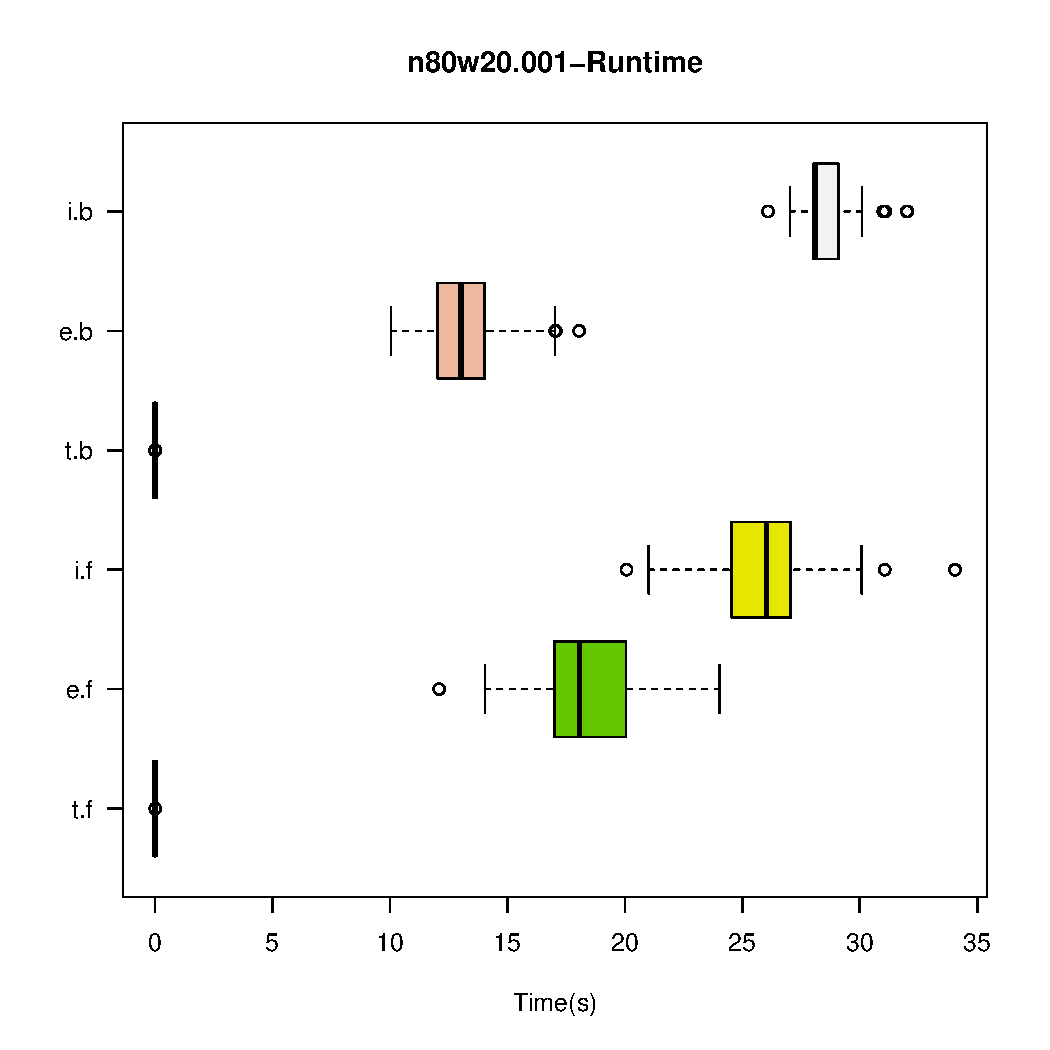
\includegraphics[width=0.6\textwidth,keepaspectratio]{{VND/n80w20.001/n80w20.001-CpuTime}.pdf}
% \captionof{figure}{n80w20.001 - Runtime boxplots for the different variable neighborhood descent algorithms}
% \end{center}

% \begin{center}
% 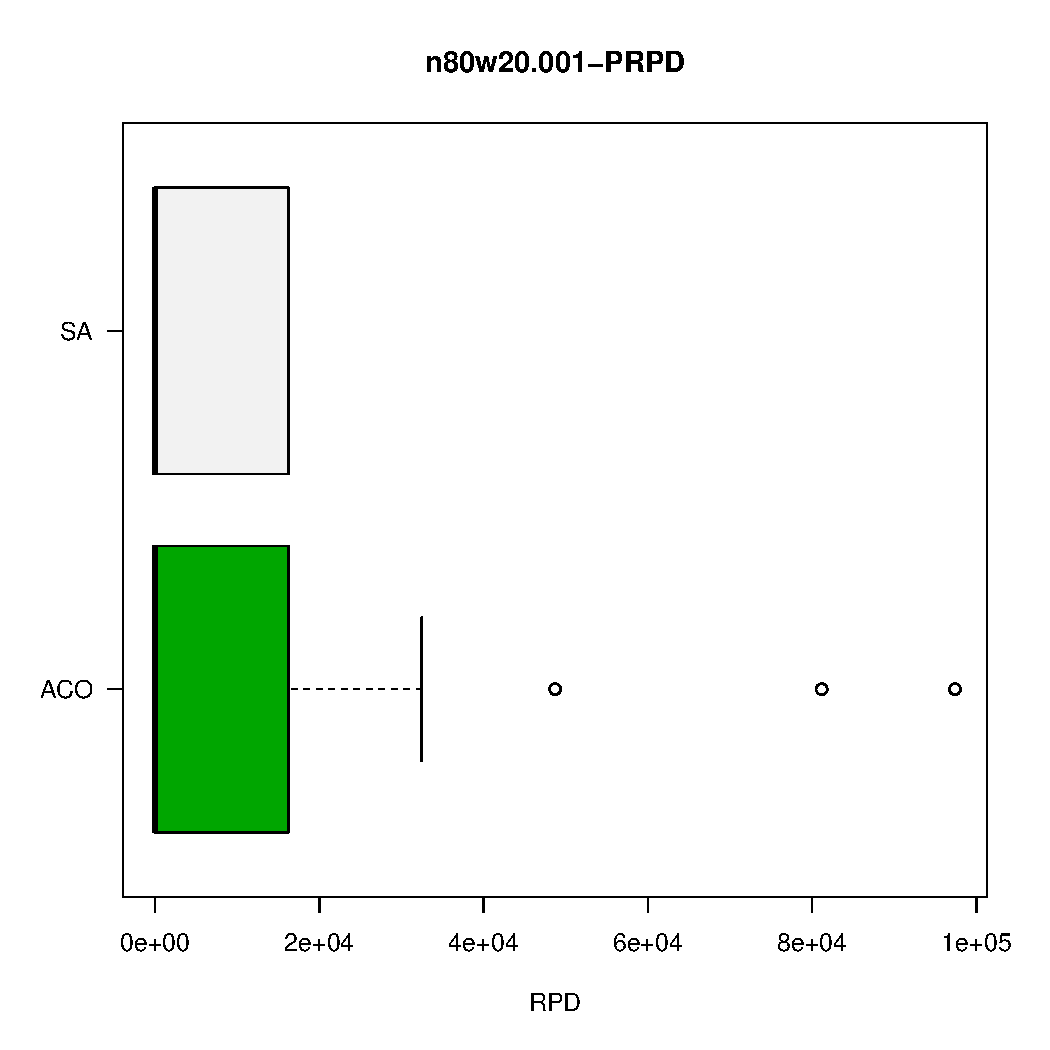
\includegraphics[width=0.6\textwidth,keepaspectratio]{{VND/n80w20.001/n80w20.001-PRPD}.pdf}
% \captionof{figure}{n80w20.001 - PRPD boxplots for the different variable neighborhood descent algorithms}
% \end{center}

% \begin{center}
% \begin{tabular}{|l|l|}
% \hline
% \textbf{Test} & \textbf{P-Value} \\
% \hline
% Tei vs Tie - Standard&3.95591160889952e-18\\
% \hline
% Tei vs Tie - Piped&3.9556885406462e-18\\
% \hline
% Standard vs Piped - Tei&3.95591160889952e-18\\
% \hline
% Standard vs Piped - Tie&3.95591160889952e-18\\
% \hline
% \end{tabular}
% \captionof{table}{n80w20.001 - Results of Wilcoxon paired signed rank test}
% \label{tab:w.11}
% \end{center}

% \subsubsection{n80w20.002}
% \begin{center}
% 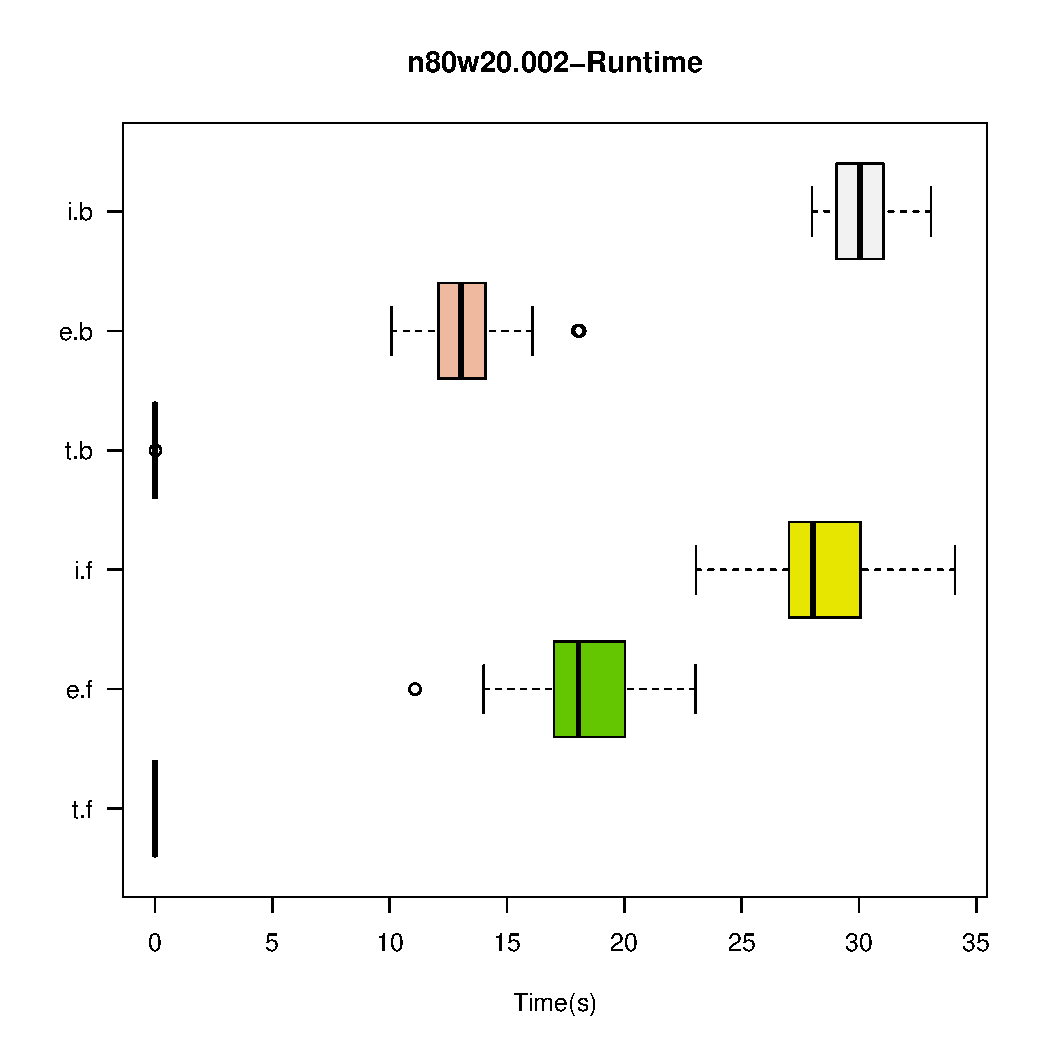
\includegraphics[width=0.6\textwidth,keepaspectratio]{{VND/n80w20.002/n80w20.002-CpuTime}.pdf}
% \captionof{figure}{n80w20.002 - Runtime boxplots for the different variable neighborhood descent algorithms}
% \end{center}

% \begin{center}
% 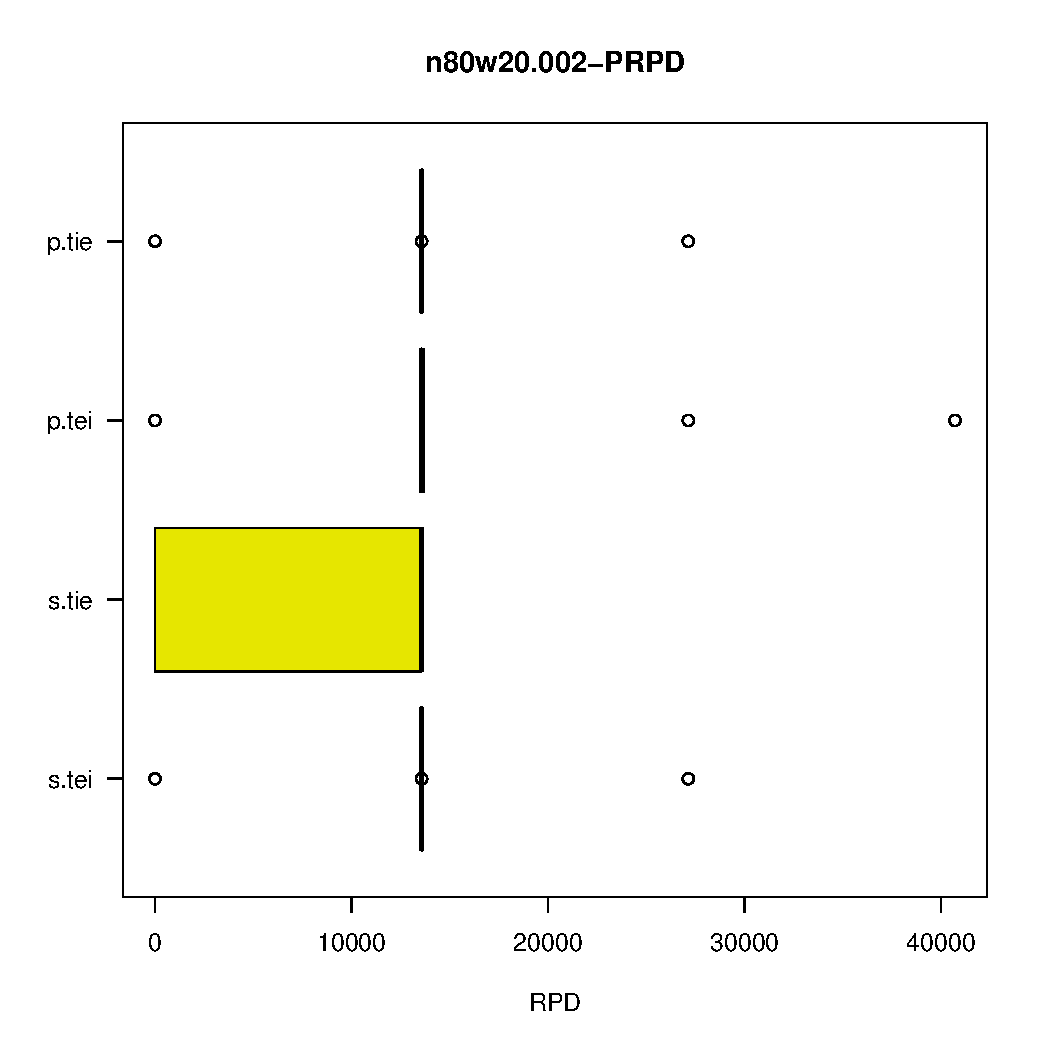
\includegraphics[width=0.6\textwidth,keepaspectratio]{{VND/n80w20.002/n80w20.002-PRPD}.pdf}
% \captionof{figure}{n80w20.002 - PRPD boxplots for the different variable neighborhood descent algorithms}
% \end{center}

% \begin{center}
% \begin{tabular}{|l|l|}
% \hline
% \textbf{Test} & \textbf{P-Value} \\
% \hline
% Tei vs Tie - Standard&3.9556885406462e-18\\
% \hline
% Tei vs Tie - Piped&3.95591160889952e-18\\
% \hline
% Standard vs Piped - Tei&3.95591160889952e-18\\
% \hline
% Standard vs Piped - Tie&3.95591160889952e-18\\
% \hline
% \end{tabular}
% \captionof{table}{n80w20.002 - Results of Wilcoxon paired signed rank test}
% \label{tab:w.12}
% \end{center}

% \subsubsection{n80w20.003}
% \begin{center}
% 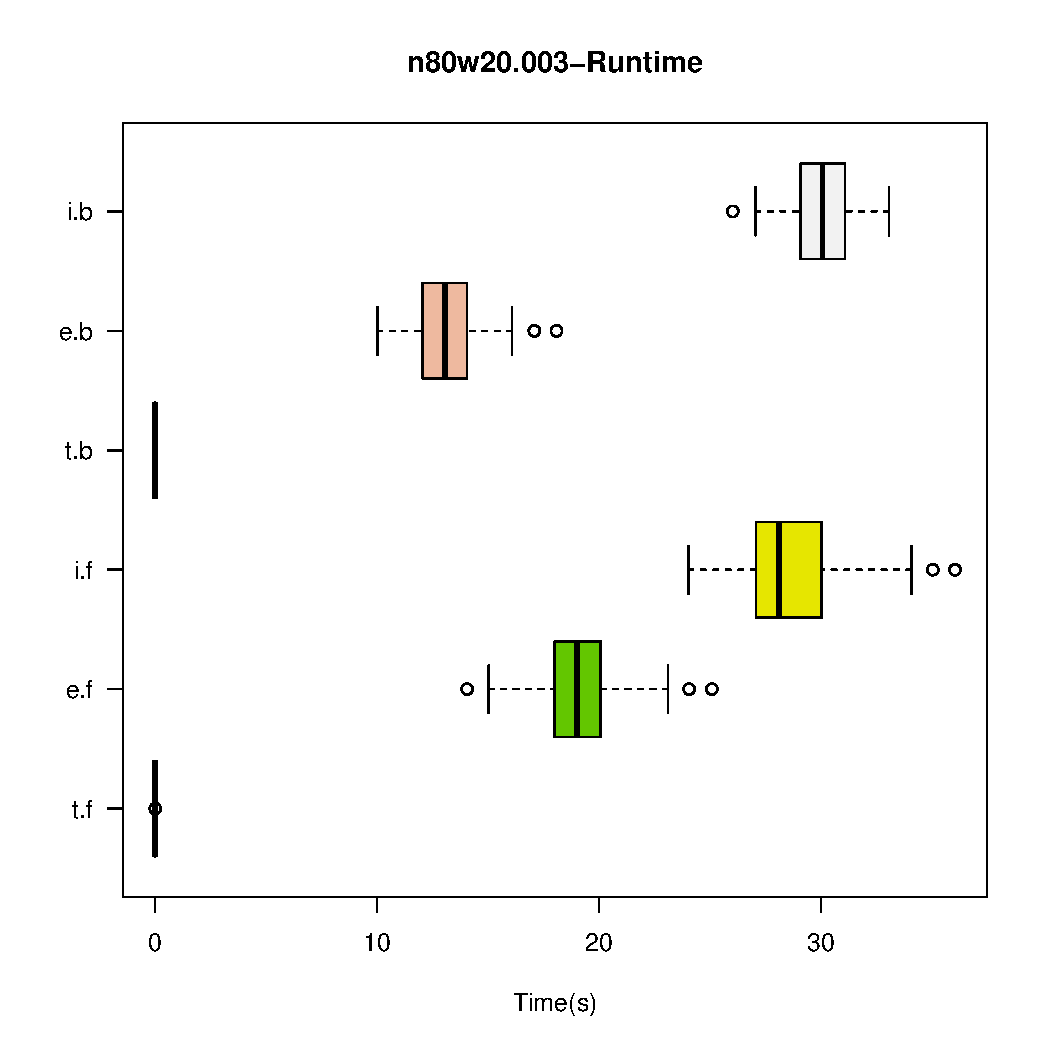
\includegraphics[width=0.6\textwidth,keepaspectratio]{{VND/n80w20.003/n80w20.003-CpuTime}.pdf}
% \captionof{figure}{n80w20.003 - Runtime boxplots for the different variable neighborhood descent algorithms}
% \end{center}

% \begin{center}
% 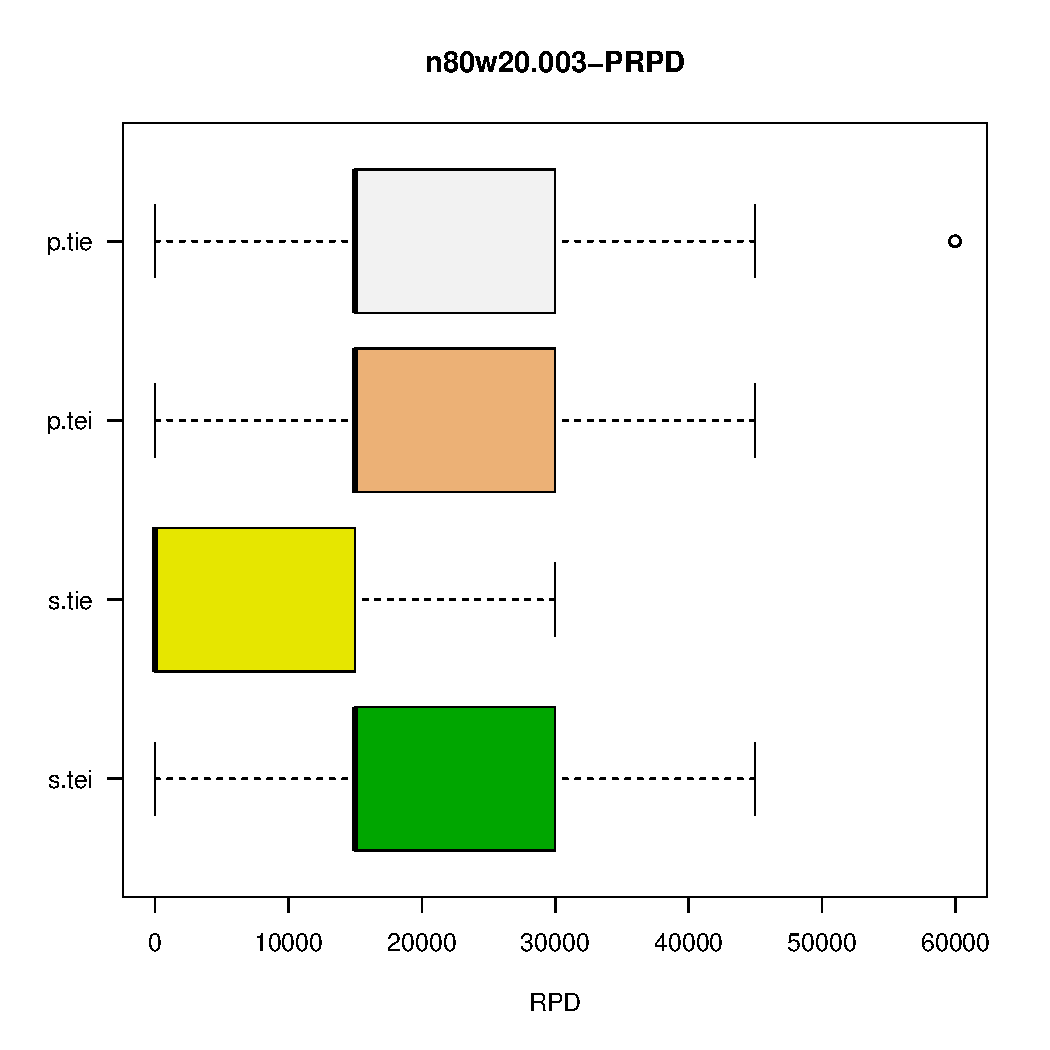
\includegraphics[width=0.6\textwidth,keepaspectratio]{{VND/n80w20.003/n80w20.003-PRPD}.pdf}
% \captionof{figure}{n80w20.003 - PRPD boxplots for the different variable neighborhood descent algorithms}
% \end{center}

% \begin{center}
% \begin{tabular}{|l|l|}
% \hline
% \textbf{Test} & \textbf{P-Value} \\
% \hline
% Tei vs Tie - Standard&3.9552424399092e-18\\
% \hline
% Tei vs Tie - Piped&3.95591160889952e-18\\
% \hline
% Standard vs Piped - Tei&3.95591160889952e-18\\
% \hline
% Standard vs Piped - Tie&3.95591160889952e-18\\
% \hline
% \end{tabular}
% \captionof{table}{n80w20.003 - Results of Wilcoxon paired signed rank test}
% \label{tab:w.13}
% \end{center}

% \subsubsection{n80w20.004}
% \begin{center}
% 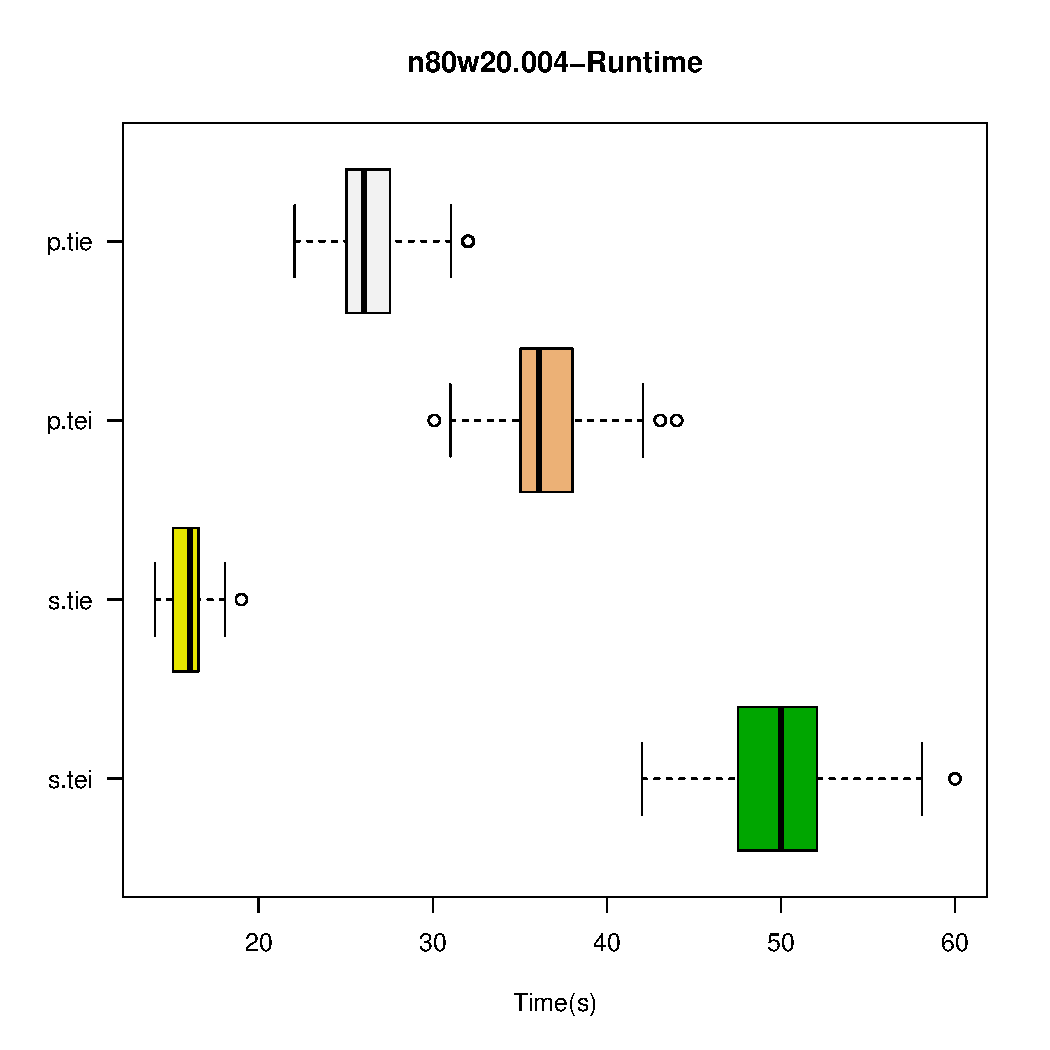
\includegraphics[width=0.6\textwidth,keepaspectratio]{{VND/n80w20.004/n80w20.004-CpuTime}.pdf}
% \captionof{figure}{n80w20.004 - Runtime boxplots for the different variable neighborhood descent algorithms}
% \end{center}

% \begin{center}
% 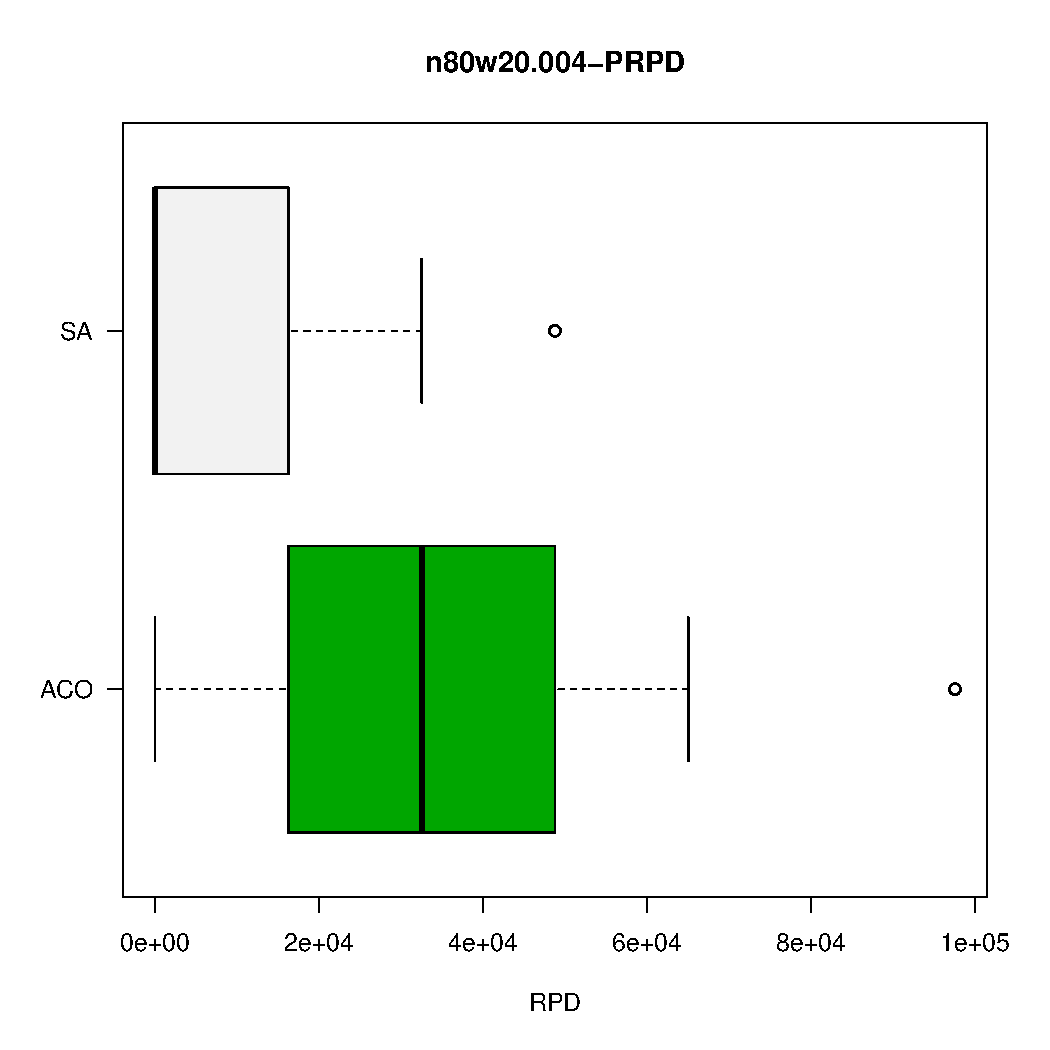
\includegraphics[width=0.6\textwidth,keepaspectratio]{{VND/n80w20.004/n80w20.004-PRPD}.pdf}
% \captionof{figure}{n80w20.004 - PRPD boxplots for the different variable neighborhood descent algorithms}
% \end{center}

% \begin{center}
% \begin{tabular}{|l|l|}
% \hline
% \textbf{Test} & \textbf{P-Value} \\
% \hline
% Tei vs Tie - Standard&3.95591160889952e-18\\
% \hline
% Tei vs Tie - Piped&3.95591160889952e-18\\
% \hline
% Standard vs Piped - Tei&3.95591160889952e-18\\
% \hline
% Standard vs Piped - Tie&3.95591160889952e-18\\
% \hline
% \end{tabular}
% \captionof{table}{n80w20.004 - Results of Wilcoxon paired signed rank test}
% \label{tab:w.14}
% \end{center}

% \subsubsection{n80w20.005}
% \begin{center}
% 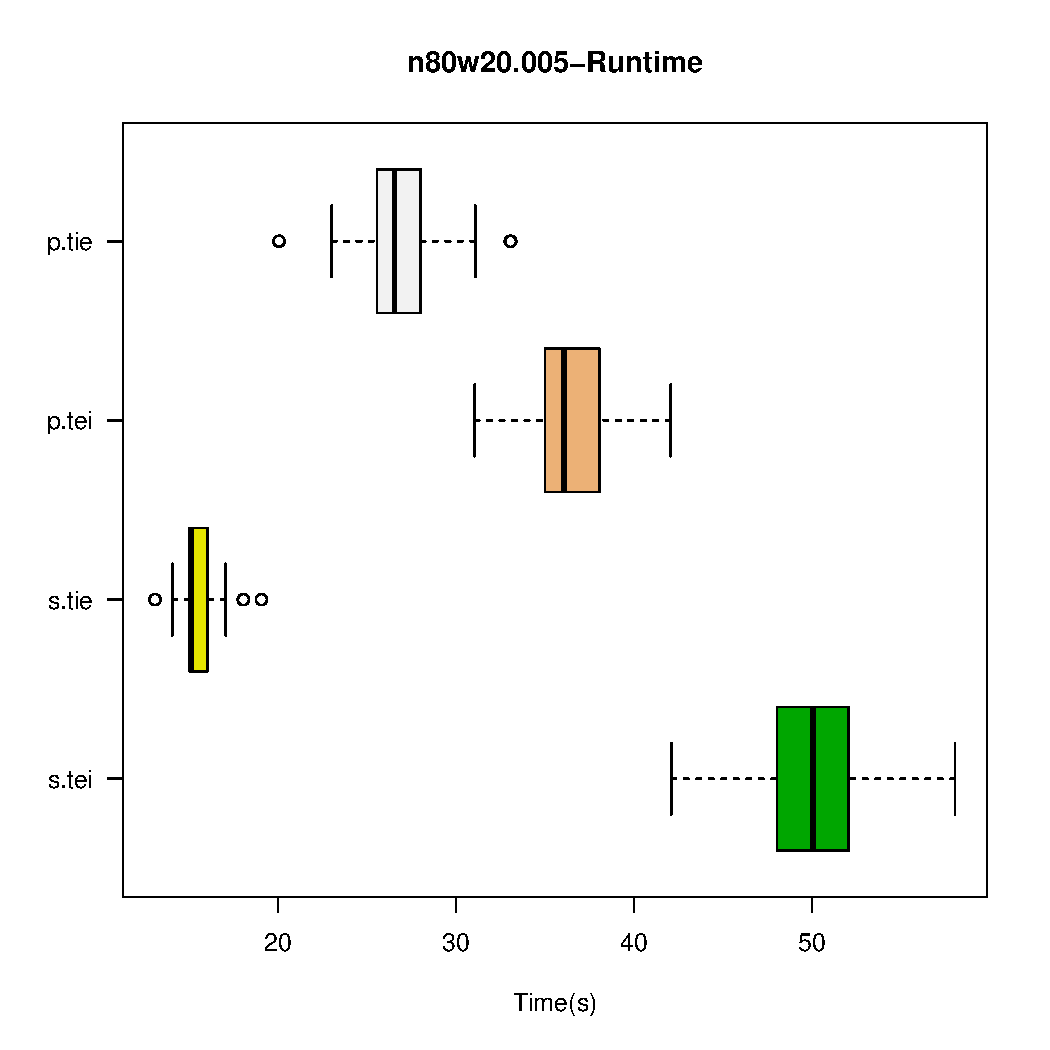
\includegraphics[width=0.6\textwidth,keepaspectratio]{{VND/n80w20.005/n80w20.005-CpuTime}.pdf}
% \captionof{figure}{n80w20.005 - Runtime boxplots for the different variable neighborhood descent algorithms}
% \end{center}

% \begin{center}
% 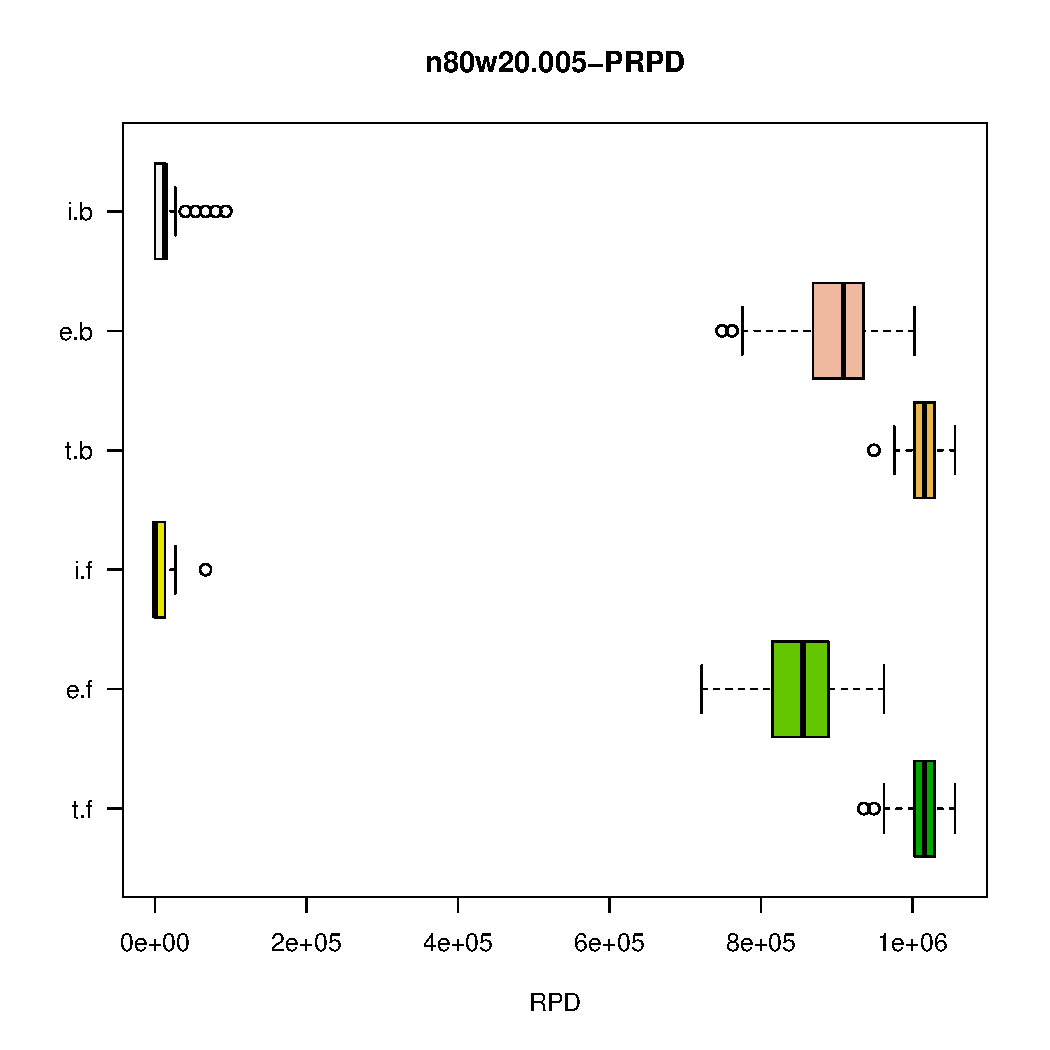
\includegraphics[width=0.6\textwidth,keepaspectratio]{{VND/n80w20.005/n80w20.005-PRPD}.pdf}
% \captionof{figure}{n80w20.001 - PRPD boxplots for the different variable neighborhood descent algorithms}
% \end{center}

% \begin{center}
% \begin{tabular}{|l|l|}
% \hline
% \textbf{Test} & \textbf{P-Value} \\
% \hline
% Tei vs Tie - Standard&3.95591160889952e-18\\
% \hline
% Tei vs Tie - Piped&3.95591160889952e-18\\
% \hline
% Standard vs Piped - Tei&3.95591160889952e-18\\
% \hline
% Standard vs Piped - Tie&3.95591160889952e-18\\
% \hline
% \end{tabular}
% \captionof{table}{n80w20.005 - Results of Wilcoxon paired signed rank test}
% \label{tab:w.15}
% \end{center}

% \subsubsection{n80w200.001}
% \begin{center}
% 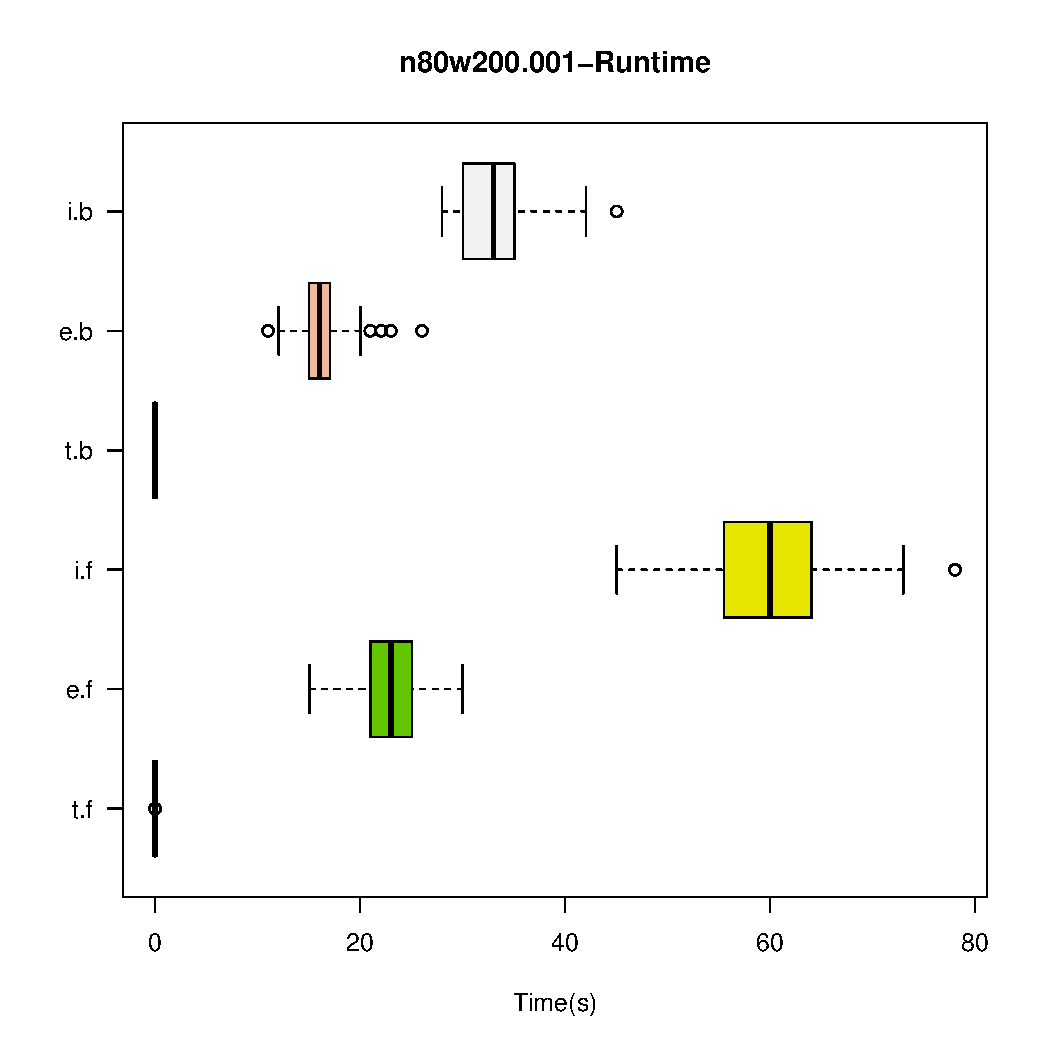
\includegraphics[width=0.6\textwidth,keepaspectratio]{{VND/n80w200.001/n80w200.001-CpuTime}.pdf}
% \captionof{figure}{n80w200.001 - Runtime boxplots for the different variable neighborhood descent algorithms}
% \end{center}

% \begin{center}
% 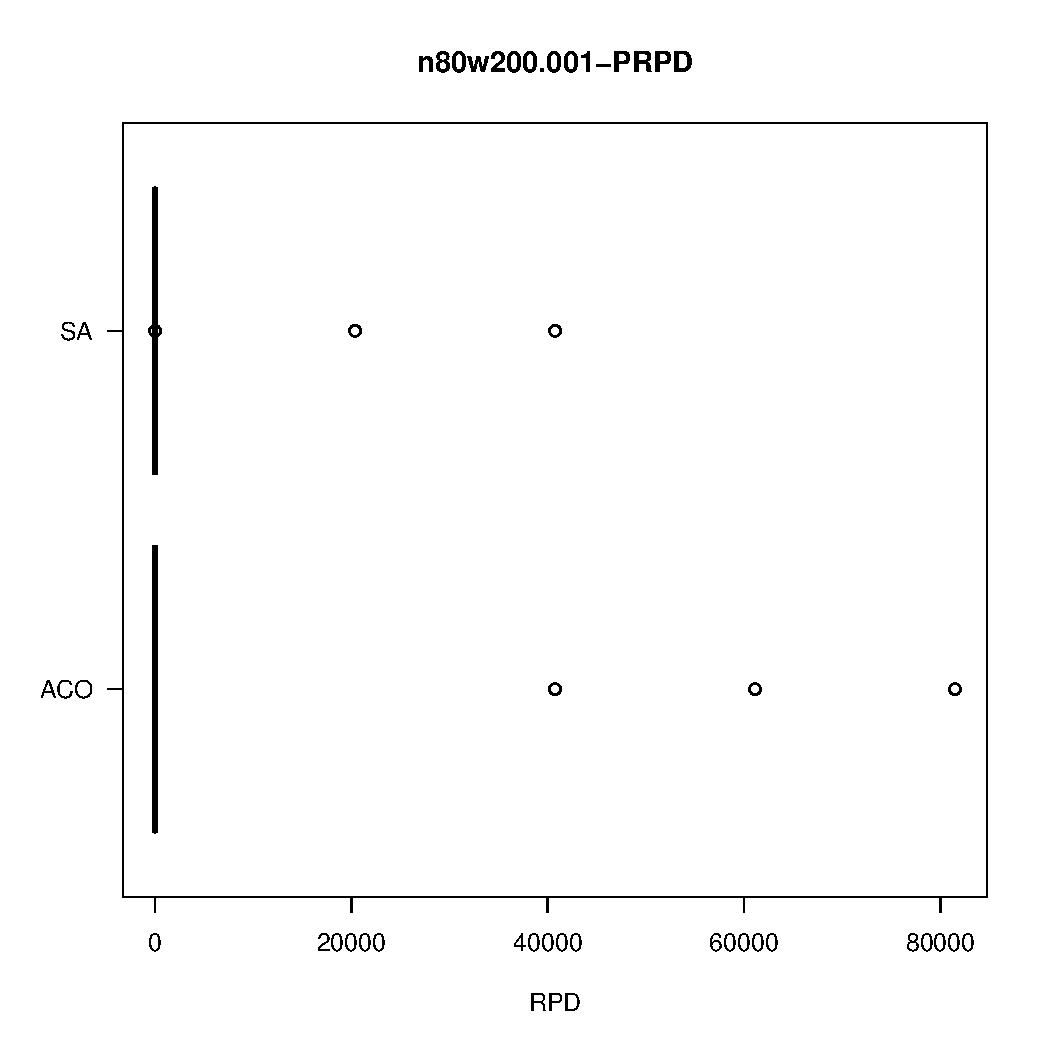
\includegraphics[width=0.6\textwidth,keepaspectratio]{{VND/n80w200.001/n80w200.001-PRPD}.pdf}
% \captionof{figure}{n80w200.001 - PRPD boxplots for the different variable neighborhood descent algorithms}
% \end{center}

% \begin{center}
% \begin{tabular}{|l|l|}
% \hline
% \textbf{Test} & \textbf{P-Value} \\
% \hline
% Tei vs Tie - Standard&4.07730530936212e-18\\
% \hline
% Tei vs Tie - Piped&2.92094064174088e-17\\
% \hline
% Standard vs Piped - Tei&2.72456795287507e-16\\
% \hline
% Standard vs Piped - Tie&3.95591160889952e-18\\
% \hline
% \end{tabular}
% \captionof{table}{n80w200.001 - Results of Wilcoxon paired signed rank test}
% \label{tab:w.16}
% \end{center}

% \subsubsection{n80w200.002}
% \begin{center}
% 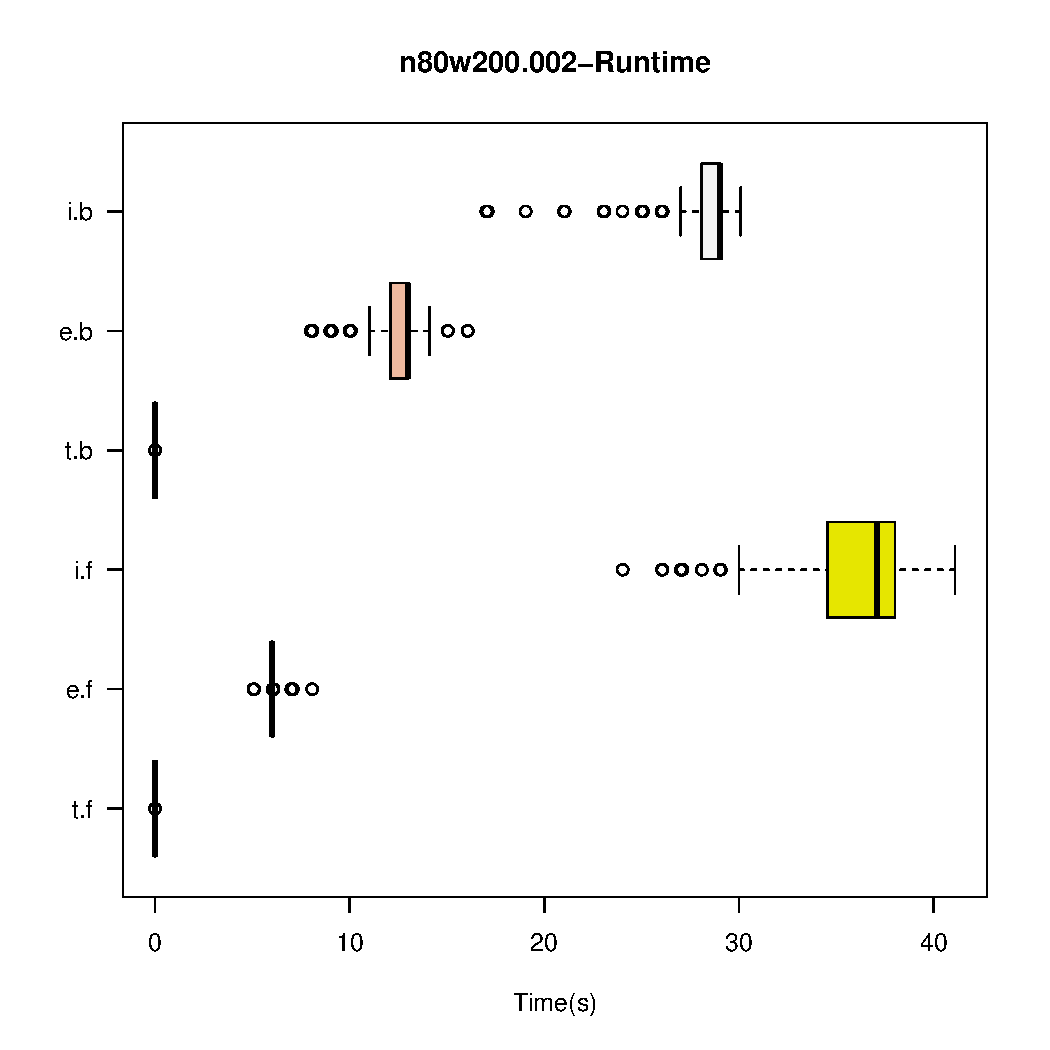
\includegraphics[width=0.6\textwidth,keepaspectratio]{{VND/n80w200.002/n80w200.002-CpuTime}.pdf}
% \captionof{figure}{n80w200.002 - Runtime boxplots for the different variable neighborhood descent algorithms}
% \end{center}

% \begin{center}
% 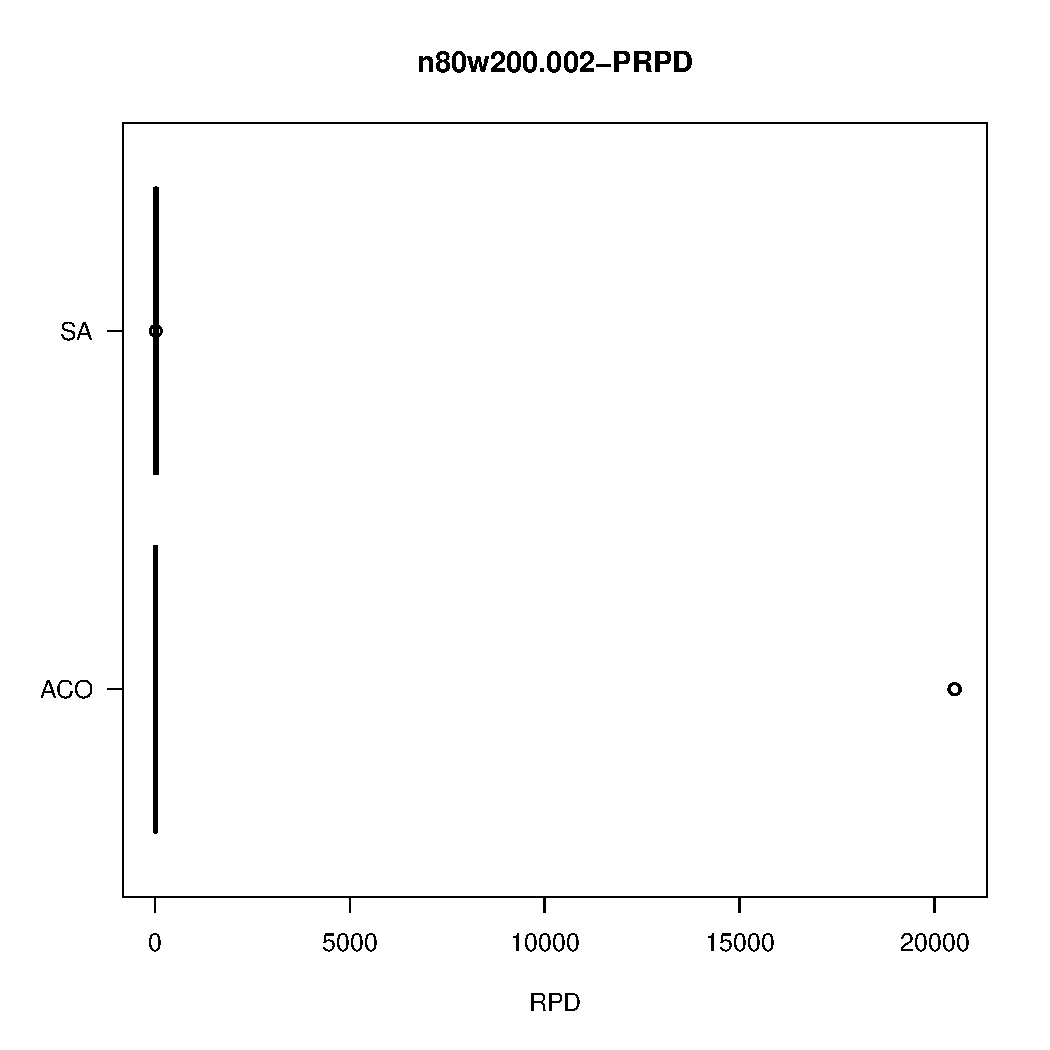
\includegraphics[width=0.6\textwidth,keepaspectratio]{{VND/n80w200.002/n80w200.002-PRPD}.pdf}
% \captionof{figure}{n80w200.002 - PRPD boxplots for the different variable neighborhood descent algorithms}
% \end{center}

% \begin{center}
% \begin{tabular}{|l|l|}
% \hline
% \textbf{Test} & \textbf{P-Value} \\
% \hline
% Tei vs Tie - Standard&3.95591160889952e-18\\
% \hline
% Tei vs Tie - Piped&1.52379449675399e-17\\
% \hline
% Standard vs Piped - Tei&1.74838327736385e-15\\
% \hline
% Standard vs Piped - Tie&3.95591160889952e-18\\
% \hline
% \end{tabular}
% \captionof{table}{n80w200.002 - Results of Wilcoxon paired signed rank test}
% \label{tab:w.17}
% \end{center}

% \subsubsection{n80w200.003}
% \begin{center}
% 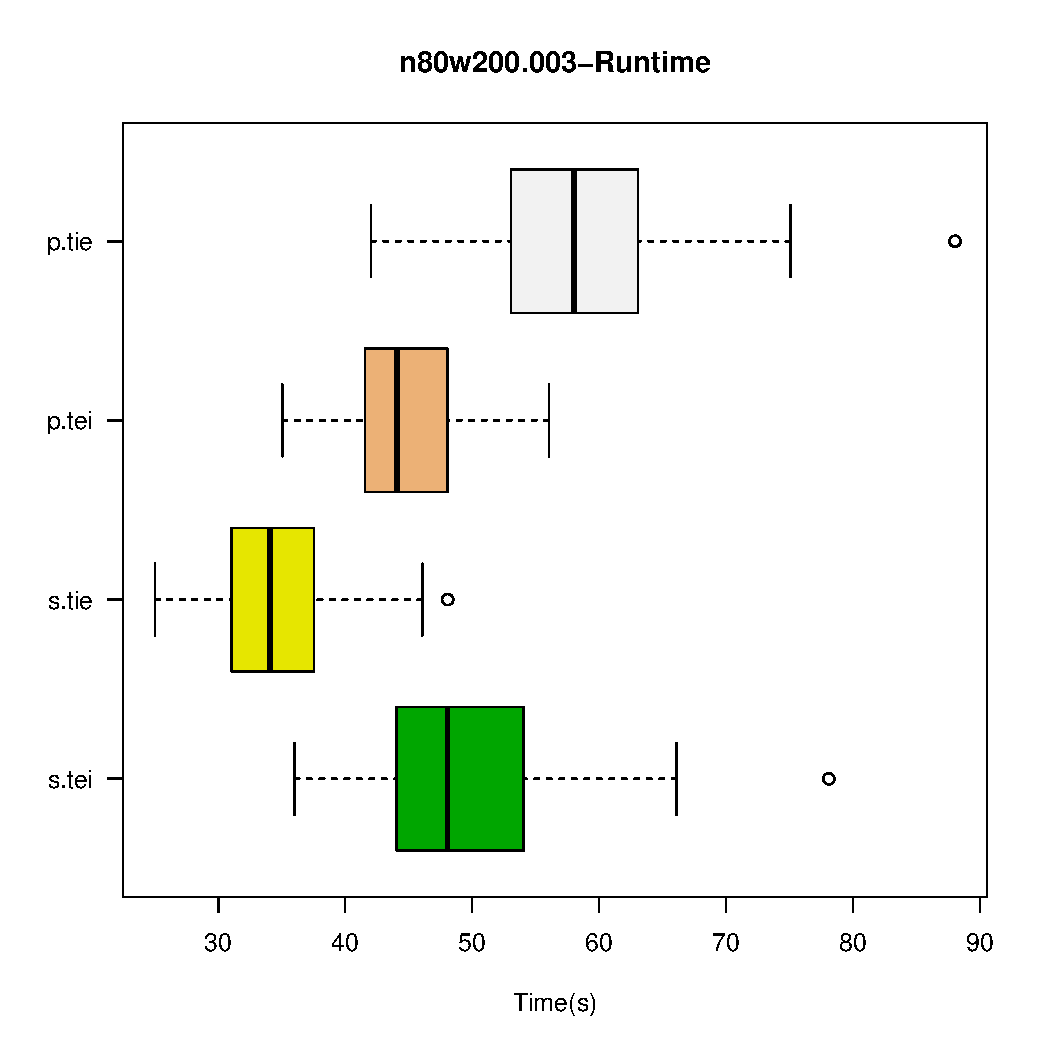
\includegraphics[width=0.6\textwidth,keepaspectratio]{{VND/n80w200.003/n80w200.003-CpuTime}.pdf}
% \captionof{figure}{n80w200.003 - Runtime boxplots for the different variable neighborhood descent algorithms}
% \end{center}

% \begin{center}
% 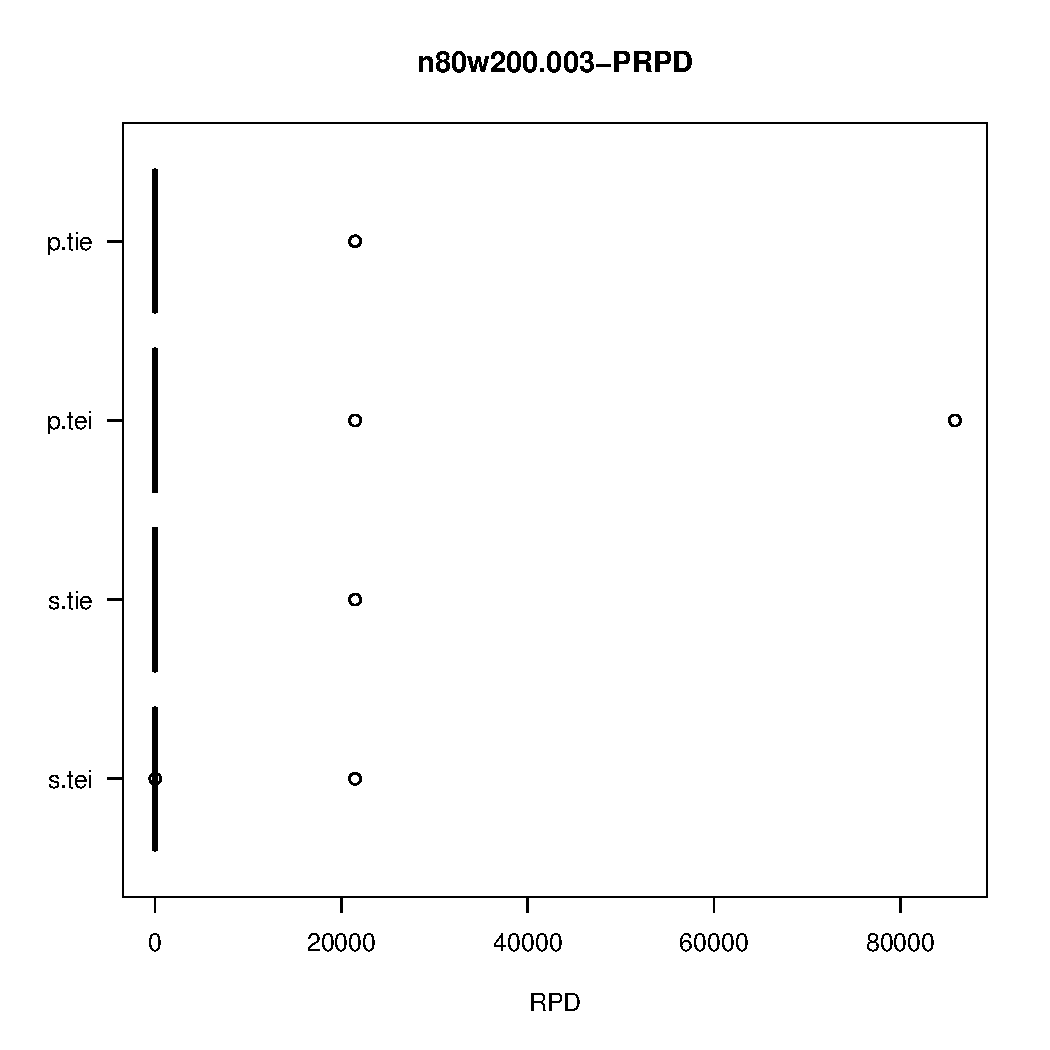
\includegraphics[width=0.6\textwidth,keepaspectratio]{{VND/n80w200.003/n80w200.003-PRPD}.pdf}
% \captionof{figure}{n80w200.003 - PRPD boxplots for the different variable neighborhood descent algorithms}
% \end{center}

% \begin{center}
% \begin{tabular}{|l|l|}
% \hline
% \textbf{Test} & \textbf{P-Value} \\
% \hline
% Tei vs Tie - Standard&2.04955667109233e-17\\
% \hline
% Tei vs Tie - Piped&2.59611565456869e-17\\
% \hline
% Standard vs Piped - Tei&1.50422804122146e-07\\
% \hline
% Standard vs Piped - Tie&3.95591160889952e-18\\
% \hline
% \end{tabular}
% \captionof{table}{n80w200.003 - Results of Wilcoxon paired signed rank test}
% \label{tab:w.18}
% \end{center}

% \subsubsection{n80w200.004}
% \begin{center}
% 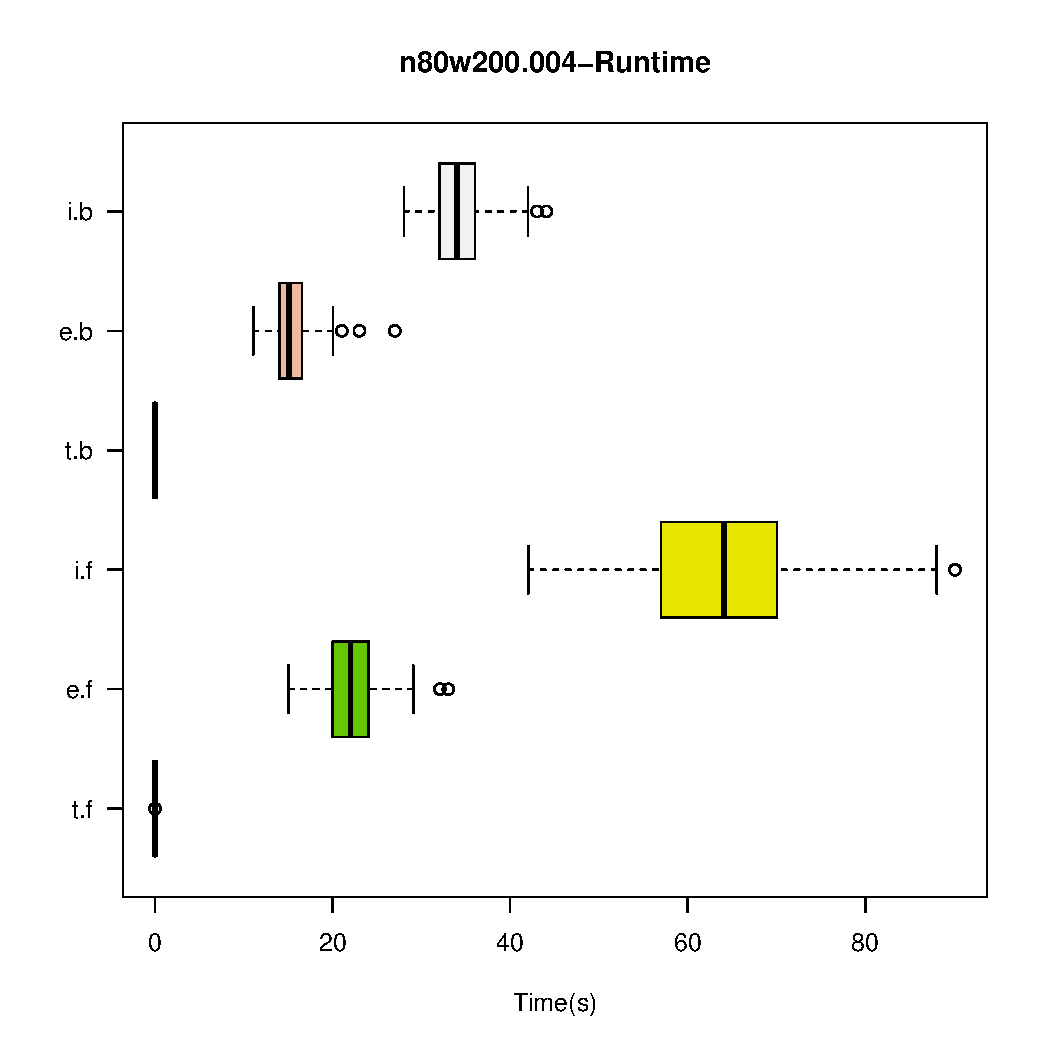
\includegraphics[width=0.6\textwidth,keepaspectratio]{{VND/n80w200.004/n80w200.004-CpuTime}.pdf}
% \captionof{figure}{n80w200.004 - Runtime boxplots for the different variable neighborhood descent algorithms}
% \end{center}

% \begin{center}
% 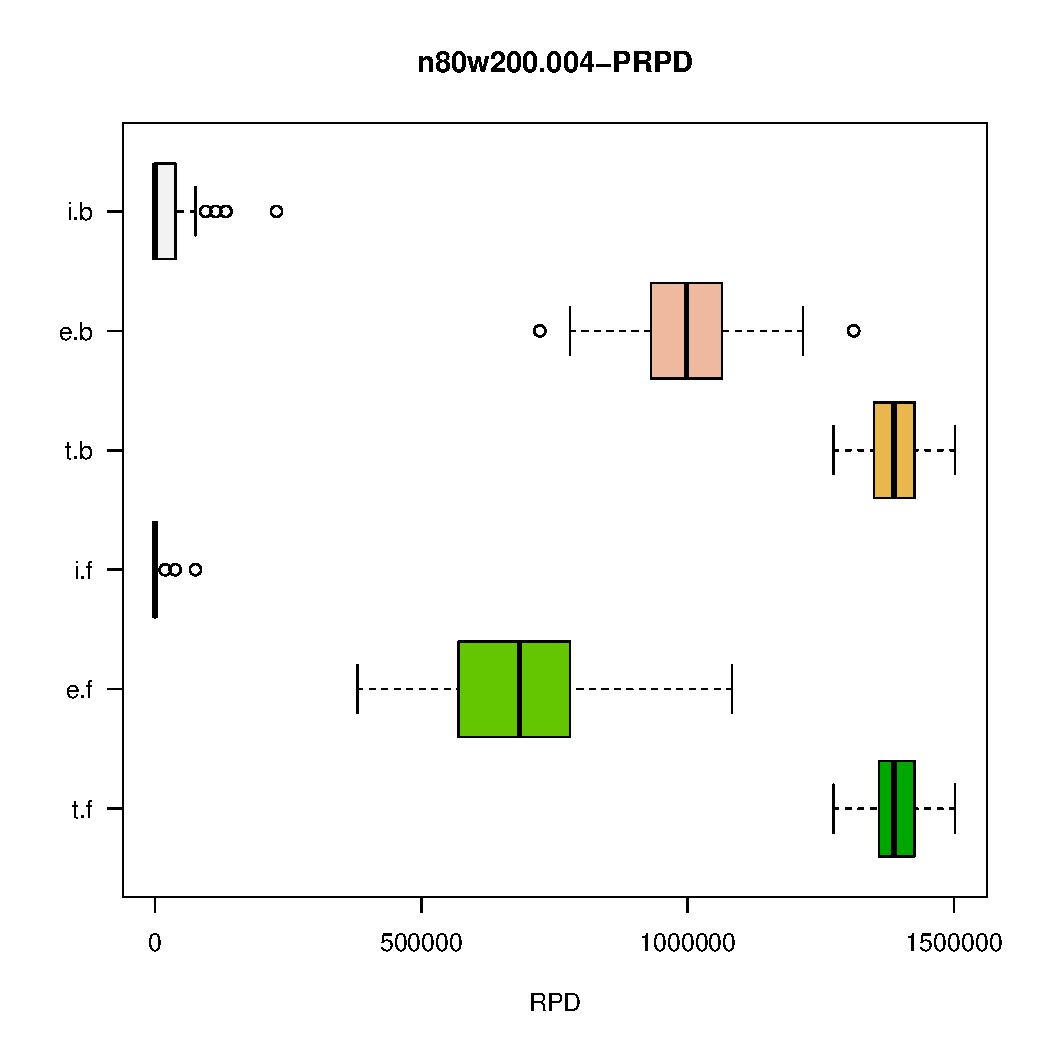
\includegraphics[width=0.6\textwidth,keepaspectratio]{{VND/n80w200.004/n80w200.004-PRPD}.pdf}
% \captionof{figure}{n80w200.004 - PRPD boxplots for the different variable neighborhood descent algorithms}
% \end{center}

% \begin{center}
% \begin{tabular}{|l|l|}
% \hline
% \textbf{Test} & \textbf{P-Value} \\
% \hline
% Tei vs Tie - Standard&4.07730530936212e-18\\
% \hline
% Tei vs Tie - Piped&4.29577057320019e-16\\
% \hline
% Standard vs Piped - Tei&5.3075517052254e-11\\
% \hline
% Standard vs Piped - Tie&3.95591160889952e-18\\
% \hline
% \end{tabular}
% \captionof{table}{n80w200.004 - Results of Wilcoxon paired signed rank test}
% \label{tab:w.19}
% \end{center}

% \subsubsection{n80w200.005}
% \begin{center}
% 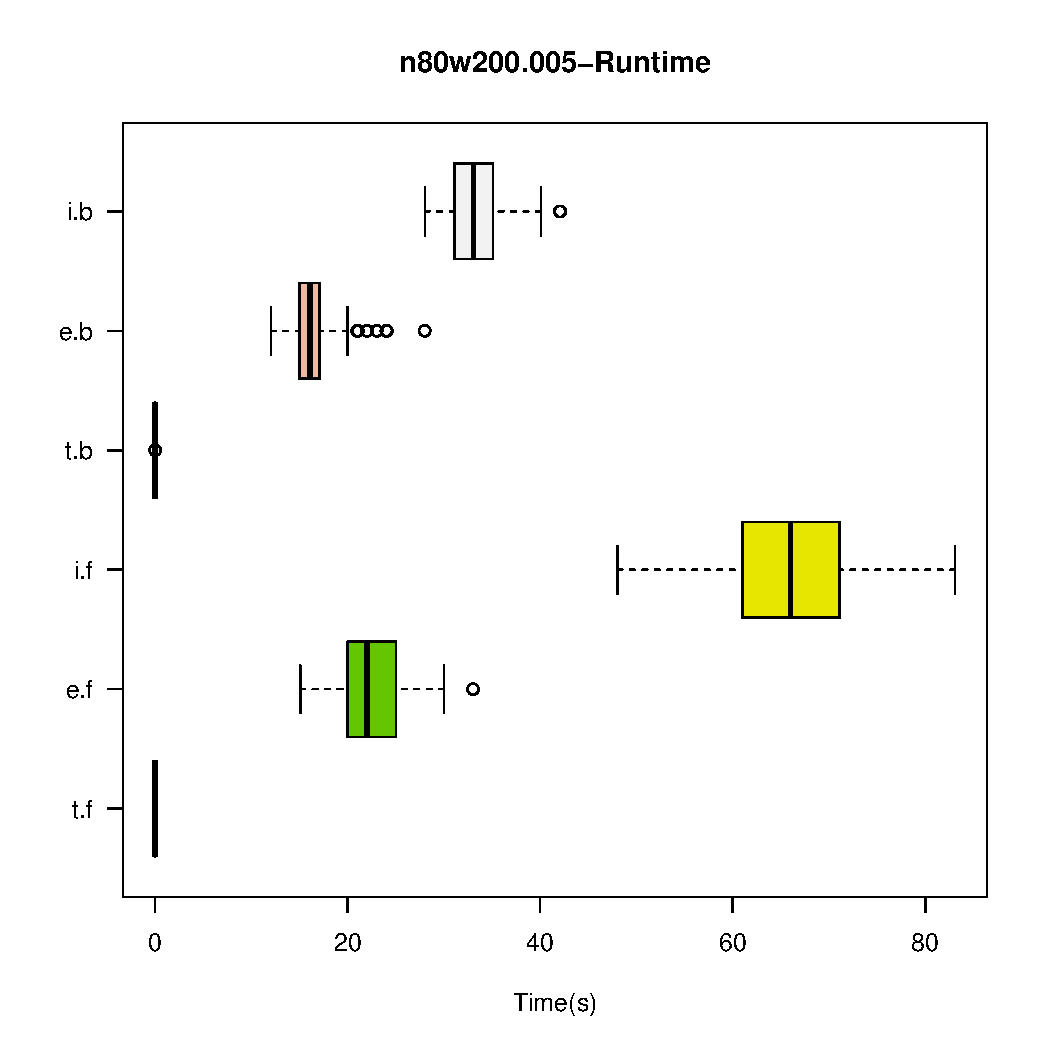
\includegraphics[width=0.6\textwidth,keepaspectratio]{{VND/n80w200.005/n80w200.005-CpuTime}.pdf}
% \captionof{figure}{n80w200.005 - Runtime boxplots for the different variable neighborhood descent algorithms}
% \end{center}

% \begin{center}
% 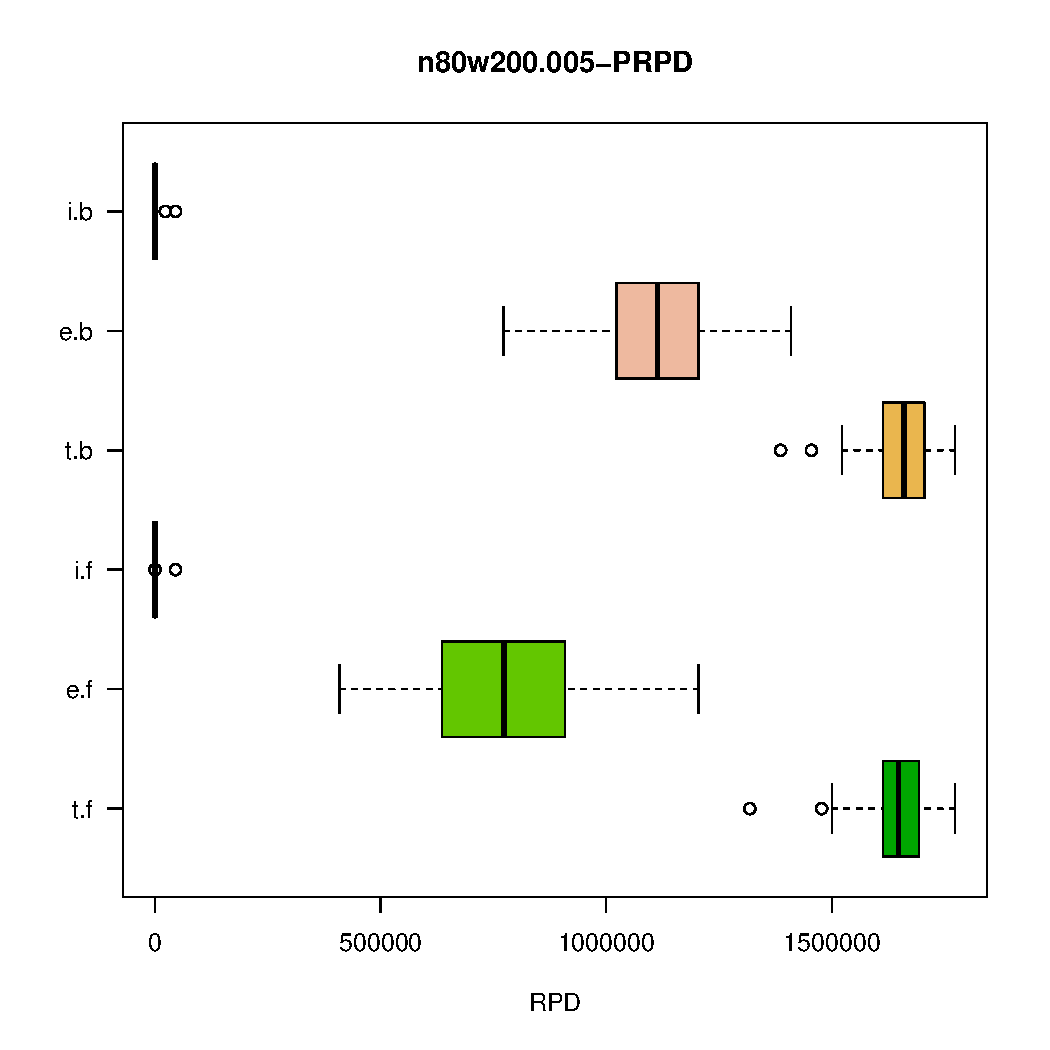
\includegraphics[width=0.6\textwidth,keepaspectratio]{{VND/n80w200.005/n80w200.005-PRPD}.pdf}
% \captionof{figure}{n80w200.001 - PRPD boxplots for the different variable neighborhood descent algorithms}
% \end{center}

% \begin{center}
% \begin{tabular}{|l|l|}
% \hline
% \textbf{Test} & \textbf{P-Value} \\
% \hline
% Tei vs Tie - Standard&1.39380002081336e-17\\
% \hline
% Tei vs Tie - Piped&4.07730530936212e-18\\
% \hline
% Standard vs Piped - Tei&3.72316935219101e-06\\
% \hline
% Standard vs Piped - Tie&3.95591160889952e-18\\
% \hline
% \end{tabular}
% \captionof{table}{n80w200.001 - Results of Wilcoxon paired signed rank test}
% \label{tab:w.20}
% \end{center}

% \subsection{Statistics}
% \subsubsection{Standard-Transpose-Exchange-Insert}
% \begin{center}
% \begin{tabular}{|l|c|l|l|}
% \hline
% \textbf{Instance}& \textbf{\% Infeasible} & $\mathbf{\bar{PRDP}}$ &$\mathbf{\bar{Runtime}}$\\
% \hline
% n80w20.001&0.71&14772.04644164&50.611339\\
% \hline
% n80w20.002&0.88&12888.542&50.727053\\
% \hline
% n80w20.003&0.92&19936.872&50.820348\\
% \hline
% n80w20.004&0.62&17234.94260984&50.049484\\
% \hline
% n80w20.005&0.94&12564.0560428&50.269182\\
% \hline
% n80w200.001&0.28&11212.97389136&49.151249\\
% \hline
% n80w200.002&0.03&629.5853274&51.433949\\
% \hline
% n80w200.003&0.07&1511.56628539&49.082085\\
% \hline
% n80w200.004&0.16&4193.4817209&49.662512\\
% \hline
% n80w200.005&0.01&466.6729061&46.701953\\
% \hline
% \end{tabular}
% \captionof{table}{Statistics summary for variable neighborhood descent algorithm with Transpose-Exchange-Insert neighborhood chain and Standard VND type}
% \label{tab:s.tei}
% \end{center}

% \subsubsection{Standard-Transpose-Insert-Exchange}
% \begin{center}
% \begin{tabular}{|l|c|l|l|}
% \hline
% \textbf{Instance}& \textbf{\% Infeasible} & $\mathbf{\bar{PRDP}}$ &$\mathbf{\bar{Runtime}}$\\
% \hline
% n80w20.001&0.54&10874.77632472&15.268454\\
% \hline
% n80w20.002&0.62&8411.724&15.386641\\
% \hline
% n80w20.003&0.44&7645.295&15.638153\\
% \hline
% n80w20.004&0.39&7153.68881324&15.980347\\
% \hline
% n80w20.005&0.25&3475.2731712&15.55767\\
% \hline
% n80w200.001&0.16&4898.3227617&33.424555\\
% \hline
% n80w200.002&0&11.0430351&32.198479\\
% \hline
% n80w200.003&0.05&1082.1460308&34.345522\\
% \hline
% n80w200.004&0.28&7804.19186258&32.583152\\
% \hline
% n80w200.005&0&10.20227353&34.501294\\
% \hline
% \end{tabular}
% \captionof{table}{Statistics summary for variable neighborhood descent algorithm with Transpose-Insert-Exchange neighborhood chain and Standard VND type}
% \label{tab:s.tie}
% \end{center}

% \subsubsection{Piped-Transpose-Exchange-Insert}
% \begin{center}
% \begin{tabular}{|l|c|l|l|}
% \hline
% \textbf{Instance}& \textbf{\% Infeasible} & $\mathbf{\bar{PRDP}}$ &$\mathbf{\bar{Runtime}}$\\
% \hline
% n80w20.001&0.59&12336.84228578&35.694416\\
% \hline
% n80w20.002&0.94&15603.0142035&36.212393\\
% \hline
% n80w20.003&0.83&19338.924&34.821217\\
% \hline
% n80w20.004&0.55&13170.33921962&36.438959\\
% \hline
% n80w20.005&0.45&6683.336214&36.202891\\
% \hline
% n80w200.001&0.19&5104.3621015&40.772642\\
% \hline
% n80w200.002&0.01&218.8179842&44.241593\\
% \hline
% n80w200.003&0.06&2584.90674231&44.725066\\
% \hline
% n80w200.004&0.17&3430.64506042&43.760992\\
% \hline
% n80w200.005&0.02&693.0136326&42.646023\\
% \hline
% \end{tabular}
% \captionof{table}{Statistics summary for variable neighborhood descent algorithm with Transpose-Exchange-Insert neighborhood chain and Piped VND type}
% \label{tab:p.tei}
% \end{center}

% \subsubsection{Piped-Transpose-Insert-Exchange}
% \begin{center}
% \begin{tabular}{|l|c|l|l|}
% \hline
% \textbf{Instance}& \textbf{\% Infeasible} & $\mathbf{\bar{PRDP}}$ &$\mathbf{\bar{Runtime}}$\\
% \hline
% n80w20.001&0.68&16393.81210394&24.788225\\
% \hline
% n80w20.002&0.81&11667.654&25.902581\\
% \hline
% n80w20.003&0.84&20537.669&26.442309\\
% \hline
% n80w20.004&0.46&8779.79314651&26.424231\\
% \hline
% n80w20.005&0.24&3876.3661498&26.511156\\
% \hline
% n80w200.001&0.21&5917.0312803&52.302366\\
% \hline
% n80w200.002&0.01&626.0983757&56.238843\\
% \hline
% n80w200.003&0.04&867.92563269&58.498874\\
% \hline
% n80w200.004&0.28&6281.58944822&55.867038\\
% \hline
% n80w200.005&0.01&236.8657243&58.331595\\
% \hline
% \end{tabular}
% \captionof{table}{Statistics summary for variable neighborhood descent algorithm with Transpose-Insert-Exchange neighborhood chain and Piped VND type}
% \label{tab:p.tie}
% \end{center}

\subsection{Results discussion}
By looking at tables \ref{tab:s.tei}, \ref{tab:s.tie}, \ref{tab:p.tei}, \ref{tab:p.tie} one can see that:
\begin{itemize}

\item For some instances (e.g. $n80w20.002$,$n80w20.003$) the algorithm are not able to converge to a feasible solution, as shown in the corresponding boxplots, since the PRPD distribution is centered around 12000-15000, thus indicating the presence of at least 1 constraint violations in most of the cases.

\item For some other instances (e.g. $n80w20.004$,$n80w20.005$) the algorithms are able to converge to feasible solutions and to the best-known one, but having a right-skewed distribution towards higher values of PRPD.

\item For the remaining instances, except for some outlier values, the algorithms are able to converge to the best-known solution in most of the runs , even though the average PRPD is not closer to 0. This is due to the fact that the mean of a distribution is sensible to outliers and the penalisation for a constraint violations is extremely high when compared to the mean value.
      
\item The algorithm ordering in terms of runtimes is $s.tie < p.tie < p.tei < s.tei$ for the  $n80w20.X$ instances while $s.tie < p.tei < s.tei < p.tie$ for $n80w200.X$ ones. The choice to explore the Insert Neighborhood before the Exchange one allows to reduce the computation time for the $n80w20.X$ instances, with a similar solution quality.

\item The algorithms are more effective on the $n80w200.X$ instances then the $n80w20.X$ once, since they have a lower percentage of infeasible runs and a lower PRPD.

\item The standard variable neighborhood descent with Transpose-Insert-Exchange neighborhood chain (s.tie) outperforms all the other algorithms in terms of solution quality and runtime.

\item Tables \ref{tab:w.11}, \ref{tab:w.12}, \ref{tab:w.13}, \ref{tab:w.14}, \ref{tab:w.15}, \ref{tab:w.16}, \ref{tab:w.17}, \ref{tab:w.18}, \ref{tab:w.19}, \ref{tab:w.20} contain, in any case, p-values considerably smaller than the significance level ($\alpha=0.05$). 

This implies that the null hypothesis corresponding to the equality of the median values of the differences of the two distributions can be rejected, hence assessing the existence of a statistically significant difference among the solution quality generated by analyzed algorithms.

\item By looking at the Cpu time, one can see that the instances \emph{n80w20.X} have generally lower runtimes than the \emph{n80w200.X} ones. They can then be considered, with respect to the variable neighborhood descent algorithms, simpler (quickier to solve) instances with respect to the latter.

\end{itemize}

\end{homeworkProblem}
